\documentclass[a4paper, 11 pt]{article}
\input{General/Preamble} % Loads in the preamble 
\input{General/Settings} % Loads in user defined settings
\input{General/MathCommands} % Loads in user defined math commands

\begin{document}

%%% PAGE DE GARDE
\thispagestyle{empty}
\begin{center}
    \newcommand{\HRule}{\rule{\linewidth}{0.5mm}}
    
    \textsc{\LARGE École Polytechnique Fédérale de Lausanne}\\[0.5cm]
    
\includegraphics[width=5cm]{Figures/epfl_red.png}\\[0.5cm]
    \LARGE{\textsc{Robotique, 2025-26}}\\[0.5cm]
    \huge{\textbf{Master thesis}}
    
    \HRule \\[0.4cm]
    {\huge \bfseries DASH-01 :\\ RL Framework to Develop a Bipedal Humanoid Robot Aimed at Breaking the Speed Record}\\[0.1cm]
    \HRule \\[0.5cm]
    \LARGE{\textsc{REHAssist} \\
    \text{13.04.2025 - 04.09.2025}}\\[0.5cm]
    
    \vspace{5mm}
    %\includegraphics[scale=0.6]{images/pageDeGarde.png}\\
    \vspace{15mm}
    
    \begin{minipage}{2in} \Large
    \textbf{Author:}\\
    Nathann \textsc{Morand}\\
    Robotics M.Sc.
    \end{minipage}
    \hfill
    \begin{minipage}{2.1in} \Large
    \textbf{Supervisors:}\\
    Dr. Mohamed \textsc{Bouri} \\
    \end{minipage}
\end{center}
%%%

%%% ABSTRACT, PROJECT ASSIGNMENT
{ % create local environment
\fancyhead[R]{\textsc{PROJECT ASSIGNMENT, ABSTRACT}}

\newpage
\section*{Abstract}
\addcontentsline{toc}{section}{Abstract}

\newpage
}
%%%
%%% TABLE OF CONTENTS
\newpage
\renewcommand{\contentsname}{Table of Contents} 
{
  \hypersetup{linkcolor=black}
  \tableofcontents
}
\newpage
%%%

% Creates the introduction, starting page numbering
\section{Introduction and context}
\label{sec:intro}

This chapter states the objective, the platform, and the scope that survived the year. It closes
with the contributions and a reading map. The rest of the document is then a single justification
chain: physics and measurement first, then constraints, then the design that follows from them.

\subsection{The platform and the objective}
\label{sec:intro-objective}

DASH-01 is a bipedal robot built at REHAssist. It carries two legs, six quasi-direct-drive
actuators, a parallel 4-bar knee, a passive ankle spring and a single-board computer. The hardware
budget was roughly EUR\,5000. \Cref{fig:robot} shows the machine as modelled.

The objective at kickoff was maximum running speed, with the bipedal 100\,m record as the stated
ambition. That record stands at 24.73\,s, or about 4.1\,m/s average, set by Cassie in
2022~\cite{crowley2024cassie}.

The project inherited a partially finished mechanical design. The work reported here therefore
starts at modelling, and at the selection of the non-mechanical subsystems. It then runs through
characterisation, learning and deployment. Five threads organise it:

\begin{enumerate}[leftmargin=*]
  \item finish the robot: actuator, battery, sensor and compute selection;
  \item learn reinforcement learning and the sim-to-real problem on a toy plant, while the robot
        did not yet exist;
  \item model the robot at a fidelity that policies can be trained against;
  \item characterise the physical robot, to bound the sim-to-real risk;
  \item produce a policy that works.
\end{enumerate}

\subsection{What the year changed about the objective}
\label{sec:intro-reframe}

Two facts reframed the objective. Both are stated here rather than conceded late.

\textbf{The record moves faster than one thesis.} New bipedal speed marks now appear at roughly a
monthly cadence, from teams with institutional budgets. A one-person master thesis on a ~CHF\,5000
chassis is not a credible contender on that timescale.

\textbf{The measured plant does not admit record pace.} \Cref{sec:speed-ceiling} bounds this
mechanism at about 2.7\,m/s in burst, and about 1.3\,m/s thermally sustained. The bound comes from
first principles, with no controller in the calculation. A 100\,m dash at record pace is about
25\,s of continuous running, so the sustained figure is the one that decides a record. The gap is a
factor of three, and it is mechanical.

The objective is therefore restated as a measured demonstrator plus a reusable method. The
deliverable is the chain from CAD to a trained policy, with every load-bearing number measured
rather than assumed. It includes an explicit account of the distance to the original target. The
thesis title still names the record, and \cref{sec:future} names the design changes that chasing it
would need.

\textbf{The problem this addresses.} Reinforcement learning has produced legged-locomotion results
on research platforms. Reproducing them on a new, custom, imperfectly known robot is a different
problem. The plant parameters are uncertain. The actuators hide undocumented internal control
loops. The sensors are commodity parts, and the computer is a single board. The gap between
``reinforcement learning walks in simulation'' and ``reinforcement learning walks on this robot'' is
dominated by modelling fidelity, actuator bandwidth, calibration and instrumentation. This thesis
measures each of those.

\textbf{Sensing scope.} Proprioception and one base inertial measurement unit are the only sensors.
Foot impact sensors were dropped for time rather than on evidence. The hardware provision for them
remains in place, as four analogue inputs on the sensor hat. The literature prior that foot feedback
helps convergence is therefore untested here.

\subsection{Contributions}
\label{sec:intro-contrib}

\begin{itemize}[leftmargin=*]
  \item \textbf{A CAD-to-MJCF pipeline for a leg that closes a kinematic loop}, with the
        loop-closure treatment URDF cannot express. It ships with validation tooling: analytic
        Jacobians checked against finite differences, and loop closure checked against the measured
        backdriven workspace at 2789 of 2789 poses (\cref{sec:twin}).
  \item \textbf{A measured plant} (\cref{tab:plant-id}). It covers weighed segment masses, a torque
        constant identified by a known-mass method that breaks the degeneracy between $K_t$ and
        gravity, the Bode response of the drive's internal position loop, inertial-sensor noise
        with provenance labels, loop timing and the CAN protocol. The identification also states
        what it could \emph{not} resolve.
  \item \textbf{A first-principles capability analysis} of running speed on that plant, validated
        against MuJoCo. Its mass-distribution sensitivity ranks the design levers
        (\cref{sec:speed-ceiling}).
  \item \textbf{An action-space and curriculum design} for the learned controller. The generator is
        a Fourier gait basis, re-parameterised every control step and mirrored across legs. It is
        wrapped in hard-wired and learned reflexes and a per-step residual channel, and trained
        under a base-degree-of-freedom release curriculum
        (\cref{sec:rl-cpg,sec:rl-curriculum}).
  \item \textbf{Two controlled comparisons that isolate the plant.} A generator A/B against an
        explicit-oscillator central pattern generator, on identical plants and rewards
        (\cref{sec:cpg-ab}). And a 21-gain scripted classical controller, which beats the learned
        reference on the constrained plant and fails identically on the free one
        (\cref{sec:scripted-baseline}).
  \item \textbf{A failure catalogue with measured diagnoses.} It covers reward exploits, six
        simulation artefacts that each produced a clean converged wrong result, four evaluation
        bugs, and the pitch-balance wall traced to plant statics (\cref{sec:negative}).
  \item \textbf{A deployment stack on the robot.} It is a 200\,Hz daemon on stock Linux, a web
        bring-up instrument that carried most of the measurement campaign, and a three-tier flight
        recorder with a pre-move guard. The recorder was built after a hardware failure, and
        validated by reproducing it (\cref{sec:deploy}).
  \item \textbf{Two published component databases with figure-of-merit tooling}, covering 140
        commercial actuators and roughly 430 battery cells. Both audited this robot's own hardware
        choices after the fact (\cref{sec:hw-selection}, \cref{sec:app-db}).
\end{itemize}

\subsection{Reading map}
\label{sec:intro-map}

\Cref{sec:bg} fixes the vocabulary, reads the field as six answers to one question, and sorts those
answers on seven analytical axes. It closes with the gap this work sits in, and three hypotheses.
\Cref{sec:robot} builds the robot and its digital twin, and replaces every assumed plant parameter
with a measured one. \Cref{sec:rl} develops the controller: five action spaces, one curriculum, and
the measured verdict on each. \Cref{sec:results} reports what the robot and the policies do.
\Cref{sec:discussion} measures the distance to the objective, and ranks the levers that close it.
\Cref{sec:conclusion} recaps. The appendix holds the logbook, the pipeline procedure, and the
database and configuration detail.

One motif recurs across the chapters, and it is worth naming in advance. The binding constraint
moves from the algorithm to the plant. \Cref{sec:bg} introduces it as a demand each control family
places on the hardware. \Cref{sec:robot} demonstrates it, because every measurement moved
pessimistically. \Cref{sec:rl} confirms it, because a learned controller and a scripted one hit the
same wall at the same time. \Cref{sec:discussion} quantifies it.
 
\section{Background and literature review}
\label{sec:bg}

This chapter supplies the frame in which the choices of \cref{sec:robot,sec:rl} are positionned. 
It also fixes the vocabulary, because ``stable'' carries different meanings in this field. 
It present the historical context of bipedal locomotion and sorts theses approaches on seven analytical axes. 
Finally, it narrows to the reinforcement-learning lineage this architecture belongs to.

\subsection{Definitions}
\label{sec:bg-defs}

Each historical family attempts bipedal locomotion by a different strategy. This section fixes the
vocabulary those families share, then sets out the four stability concepts the rest of the chapter
sorts them by.


A few terms recur :
\textbf{Underactuation} is the excess of degrees of freedom over actuators. 
\textbf{Unilateral contact} means a foot can push but not pull, and only inside the \textbf{friction cone}. 
The point where the push applies is the \textbf{centre of pressure}, confined to the contact patch. 
\textbf{Duty factor} is the fraction of a stride each foot spends in stance, and a \textbf{flight phase} is the interval with no foot down. 
The \textbf{sim-to-real gap} is the performance loss on transfer from a simulated plant to the physical one.
In the context of this thesis, \textbf{Failure} is episode termination on body contact, or on leaving the measured workspace. 
\textbf{Stability margin} is reported as a survivor count and a seed variance rather than as a scalar reward, for the reason given in \cref{sec:margin-analysis}.
The reference timescale is the free-topple time of the inverted pendulum, $\sqrt{h/g} \approx 310$\,ms for this robot.
\textbf{Stability} is the ability to continue locomotion when subjected to disturbances. 

\textbf{Static stability} holds when the ground projection of the centre of mass stays inside the
support polygon. It assumes quasi-static motion, flat feet and flat ground. The flat-ground
assumption is the fragile one, because on uneven terrain the support-polygon test can be arbitrarily
wrong~\cite{bretl2008static}. Static stability therefore admits only gaits slow enough for inertia to
be negligible, with at least one foot down throughout.

\textbf{Zero moment point stability} holds when the zero moment point stays inside the support
polygon~\cite{vukobratovic1969}. The criterion releases the quasi-static assumption, so the centre of
mass may travel beyond the support polygon, and it carried the field through
ASIMO~\cite{hirai1998honda}. It still assumes a contact patch of finite area, and still forbids a
flight phase. The test also stays conservative, because it reduces the dynamics to a force balance
and so admits slow motions rather than fully dynamic ones~\cite{chevallereau2003rabbit}. For a point
foot the support polygon degenerates to a point, and the test then never passes while the robot
moves. DASH-01 carries a spherical toe, so neither this nor the previous concepts applies to it.

\textbf{Orbital stability} holds when the spectral radius of the linearised Poincar\'e map falls below one.
If the point is outside the stable radius, the gait might work but is unstable to any tiny perturbation. 
It certifies a whole period of the gait instead of a single instant. 
A flight phase is admissible. It work only by assuming an
exactly known model and a fixed periodic gait, and each new gait need one offline
optimisation~\cite{westervelt2003hzd}. The map is linearised, so the certificate covers small
perturbations only. RABBIT is the point-foot biped the framework was built for~\cite{chevallereau2003rabbit}.

\textbf{Capturability} holds when a reachable foothold exists that brings the reduced model to a stop~\cite{pratt2006capture,koolen2012capturability}. 
Unlike the three previous concepts, which care about whether the present state is valid, what capturability care about is whether a
stopping option exists in the future. It need a reduced model and reachable footholds.

The field has moved down the order of the previous list over the last fifty years, releasing constraints to buy performance~\cite{wieber2016handbook,pratt2006margins,hobbelen2007lcw}.

\subsection{What makes bipedal locomotion hard}
\label{sec:bg-hard}

A legged robot touches the world only through intermittent unilateral contacts. Three consequences
follow.

\textbf{It is underactuated.} Six leg motors against twelve degrees of freedom leaves six base
degrees with no motor attached. The spring angle are not considered as DoF. Those six can be influenced only through the ground. A flight phase
has no ground, so the centre of mass follows a ballistic arc no actuation can alter, and the robot
chooses only the posture it will land in.

\textbf{The inputs are unilateral and saturating.} The centre of pressure moves only within the
contact patch, and since the robot has a point foot, the patch is a point. That leaves foot placement as the
only input. It is chosen once per step, and bounded by the leg's reachable workspace.

\textbf{The timescales are short.} An inverted pendulum of leg length $h$ diverges with time
constant $\sqrt{h/g}$, about 310\,ms in this case, and running contacts last tens of milliseconds. A
correction are time critical, which makes actuator bandwidth a major constraint since we can only react trough foot placement. \Cref{sec:plant-id-drive} measures
this robot's drive at a 0.8\,Hz pole in servo mode and 12 \,Hz in MIT mode. Attentive reader will notice the traquenard that will come back later.

\subsection{Historical context}
\label{sec:bg-history}

As explained in the Definitions section, the families below are sorted by where they get their stability from.

\textbf{Geometry.} WABOT-1 (1973) moved slowly enough for its own momentum to be
neglected~\cite{lim2007waseda}. The dynamic generalisation is the zero moment
point~\cite{vukobratovic1969,vukobratovic2004}, which carried the field for three decades through
Honda's P2 and ASIMO~\cite{hirai1998honda}. The linear inverted pendulum model made it cheap to compute~\cite{kajita2001lipm,kajita2003preview}.

\textbf{The mechanism.} McGeer's passive dynamic walkers descend a ramp passively using gravity alone ~\cite{mcgeer1990}. 
The gait is a limit cycle set by linkage geometry and mass distribution. 
Collins et al.\ added a motor to walk on a flat ground, 
and measured a cost of transport near 0.20, which is similar to humans~\cite{collins2005}.

\textbf{Foot placement.} Raibert's hoppers reframed the problem: a running robot has to be balanced
only during the stance phase rather than continuously~\cite{raibert1986}. 
Control decomposes into thrust at bottom of stance, foot placement about a neutral point, and hip torque applied during stance only.

\begin{equation}
  x_f \;=\; \tfrac{1}{2}\,\dot x\,T_s \;+\; k\,(\dot x - \dot x_d),
  \label{eq:neutral-point}
\end{equation}

$x_f$ is the fore-aft foot placement, measured from the hip at touchdown, in metres. \\
$\dot x$ is the current forward speed in metres per second. \\
$\dot x_d$ is the commanded forward speed, in metres per second.  \\
$T_s$ is the stance duration in seconds. \\
$k$ is a velocity feedback gain, also in seconds.  \\
This equation give the foot placement that will bring the robot back to the commanded speed in one step. 
The first term is the neutral point, which yield no net fore-aft impulse. 
The second term corrects for the speed : running faster than commanded places the foot further forward, so stance decelerates the body.
The lineage runs through BigDog~\cite{raibert2008bigdog} to Atlas.
This equation made the early Boston dynamics possible.

\textbf{Re-solving online. (MPC)} Wieber recycled zero-moment-point walking as model-predictive
control~\cite{wieber2006mpc} by doing on line. Kuindersma et al.\ built the whole-body version that ran Atlas at the
DARPA Robotics Challenge~\cite{kuindersma2016atlas}.

\textbf{Reinforcement learning.} A neural network learn a policy by reinforcement learning to
maximise a reward over millions of simulated episodes.
PPO~\cite{schulman2017ppo} became the workhorse, MuJoCo~\cite{todorov2012mujoco} made it computationally affordable, and
massively parallel simulation cut wall-clock further as demonstrated by Rudin et al. by training a walking policy under 4 minutes~\cite{rudin2021}. 
What used to be stability margin now show up in the form of a sim2real gap.
Previous approach yielded a fixed mathematical law that matched a specific plant (aka robot)
The RL approach allow to train against a multitude of variation of the plant to make it robust to unknown at the expense of some peak performance and more training steps.
This is called domain randomisation~\cite{tobin2017dr,tan2018sim2real}.
Teacher--student distillation~\cite{lee2020terrain,miki2022perceptive} allow to reduce the size of the final network for online inference.

\subsection{Approach comparison}
\label{sec:bg-axes}

The main difference stem between the RL approach and the rest.
Previous approach yielded a fixed mathematical law that could be analysed with the classical control toolkit.
The RL approach is more like a black box where most of the classical tool for stability analysis do not apply.


\subsection{Reinforcement learning for locomotion}
\label{sec:bg-rl-loco}

\subsubsection{Control architecture}

Several actuator-level control architectures have been used by the literature.

\textbf{Direct torque control} provides the policy with the highest level of control authority, but also imposes the most demanding communication and control-loop requirements. It is the mode the quasi-direct-drive actuator lineage was designed for~\cite{seok2015design,wensing2017proprioceptive}, and the one MIT Cheetah commands through~\cite{dicarlo2018mpc}. In simulation, the policy can directly command joint torques at a high frequency. On the physical robot, however, closing such a fast loop requires the policy, communication bus, actuator controller, and state estimation to operate with sufficiently low latency. In the present hardware architecture, this approach was not practical through the CAN communication bus at the required frequency.

\textbf{Direct position control} substantially reduces these requirements by delegating the low-level actuator dynamics to the motor controller. Position targets over a joint-level PD loop are what most learned locomotion uses~\cite{hwangbo2019anymal,tan2018sim2real,rudin2021}. Two variants were investigated: conventional smart-servo position control and the MIT control mode with fixed compliance parameters~\cite{katz2019minicheetah}. Both allow the RL policy to operate at a lower frequency while the actuator controller handles the fast inner loop.

\textbf{Impedance control} provides an intermediate level of control authority. Instead of directly specifying the actuator torque or position response, the policy can influence the desired mechanical behaviour through position, stiffness, damping, and/or torque-related parameters. The $[q_d, \dot q_d, K_p, K_d, \tau_{\text{ff}}]$ command frame established by the Cheetah lineage is the standard realisation~\cite{katz2019minicheetah,wensing2017proprioceptive}, and \cref{eq:impedance} is the form this thesis uses. This allows the low-level controller to preserve fast and stabilising actuator dynamics while giving the policy greater freedom than pure position control.

\subsubsection{Gait prior}

The second major design dimension is the amount and location of prior structure imposed on the gait.

A strong prior can be introduced through a \textbf{reference trajectory}. In this case, the policy is primarily trained to track or adapt an authored motion. DeepMimic tracks motion-capture clips this way~\cite{peng2018deepmimic}, and the Cassie line tracked authored reference motions~\cite{xie2019}. This strongly restricts the reachable set of motions and can substantially simplify learning. However, the quality of the resulting behaviour is bounded by the choice of reference: there is no guarantee that the selected trajectory is optimal for the particular robot morphology and dynamics.

A weaker prior can instead be introduced through a \textbf{trajectory generator} whose parameters are modulated by the policy~\cite{pmtg2018}. This preserves the assumption that locomotion should have a structured, periodic form while allowing the learned controller to search for a gait adapted to the plant. Trajectory generators can themselves provide different levels of freedom.

At the stronger end of this generator-based formulation, the policy only modifies a small number of \textbf{high-level gait parameters}, such as phase, frequency, stride length, or amplitude~\cite{pmtg2018,cpgrl2022}. Central pattern generators are the classical form of that prior~\cite{ijspeert2008}, and dynamical movement primitives the classical form for non-periodic motions~\cite{ijspeert2013dmp}. The shape of the individual joint trajectories remains largely prescribed. This provides a relatively small search space but limits the set of gaits that can be represented.

A weaker prior allows the policy to modify the \textbf{complete trajectory}. Rather than predicting every trajectory sample independently, the possible trajectories can be represented using a low-dimensional basis, such as Fourier series~\cite{shafii2010tfs,yang2010tfs,wang2023fourier,fld2024} or Bézier curves~\cite{westervelt2007book,castillo2020hzdrl}. The policy then modifies the coefficients of this representation. This retains useful structural assumptions, most importantly periodicity and smoothness, while allowing the shape of the gait itself to become a learned variable.

At the extreme, \textbf{no explicit gait prior} is imposed and the policy directly learns the complete joint trajectory~\cite{heess2017emergence,radosavovic2024humanoid}. Periodic locomotion can still be encouraged through reward shaping, but periodicity then becomes an emergent property rather than a constraint. Such an approach provides a large reachable set but considerably increases the exploration and learning problem, and there is no guarantee that the learned solution will converge to a periodic gait.

This distinction is important because the periodicity prior is not unique to the present framework. It can be introduced at different levels: through the \textbf{reward}~\cite{siekmann2021}, through a \textbf{reference motion}~\cite{peng2018deepmimic}, through an authored \textbf{trajectory generator}~\cite{pmtg2018,cpgrl2022}, or directly through the \textbf{action space} by parameterising the trajectory itself~\cite{fld2024,ates2025freqgait}. These choices determine how much of the gait is fixed and how much is available to the policy at run time.

\subsubsection{Choice for DASH-01}

For DASH-01, a fully unconstrained joint-level policy was considered undesirable because it would require reinforcement learning to simultaneously discover both the appropriate periodic structure of the gait and the stabilising behaviour of the robot. Conversely, imposing a fixed reference trajectory would strongly constrain the solution and assume that a sufficiently good gait was already known.

DASH-01 also does not correspond closely to a particular biological morphology. Consequently, transferring a reference trajectory derived from human or animal locomotion would introduce a potentially unjustified assumption about the optimal gait. A trajectory generator therefore provides a useful intermediate solution: the existence of a periodic gait is used as a prior, while its detailed shape remains a decision variable for the policy.

The framework consequently investigates a \textbf{Fourier-based gait parameterisation}, in which the joint trajectories over a gait cycle are represented by Fourier coefficients. The policy can modify these coefficients to search for a gait adapted to the specific morphology and dynamics of DASH-01. This reduces the dimensionality and imposes smooth periodic structure compared with a fully free trajectory representation, while retaining substantially more freedom than tracking a fixed reference trajectory.

The use of a Fourier representation should not itself be interpreted as the contribution of this work. Fourier-based periodic trajectory representations and the use of basis coefficients for locomotion predate this framework. The contribution of the framework instead lies in how the gait parameterisation is integrated with reinforcement learning and fast feedback control, and in the experimental comparison of alternative parameterisations under equivalent conditions.

In particular, the framework distinguishes between the \textbf{slow gait-generation channel} and the \textbf{fast feedback channel}. The gait parameters determine the underlying periodic motion, while the feedback component is responsible for reacting to disturbances and short-timescale deviations from that nominal gait. This separation allows the learned policy to modify the gait without requiring it to reconstruct the complete high-frequency actuator behaviour at every timestep.

The choice of this architecture was therefore motivated by a trade-off between \textbf{reachable gait space and learning complexity}. A fixed reference trajectory provides a strong prior but may exclude the optimal gait. A completely free policy provides a very weak prior but greatly increases the search space. A parameterised trajectory generator occupies an intermediate position: it constrains the search to smooth periodic motions while allowing the gait itself to be discovered by reinforcement learning.

\subsubsection{Architectures investigated}

Because the original objective of the thesis was to develop an RL framework capable of producing high-speed bipedal locomotion, these architectural choices were treated as experimental design variables rather than assumptions fixed from the outset.

Multiple actuator and gait-control architectures were therefore implemented and evaluated during framework development. These included direct position control, MIT-mode control with fixed compliance parameters, impedance-based control, gait-generator approaches with different levels of policy authority, and architectures incorporating a hand-tuned reflex controller alongside the learned component.

The final architecture was selected based on the resulting trade-off between actuator controllability, communication and bandwidth requirements, exploration complexity, and the freedom available to discover a gait adapted to DASH-01. The Fourier gait representation should consequently be understood as the selected design point within this broader architectural investigation, rather than as a novel gait representation in itself.


A \textbf{shape prior} fixes the trajectory and exposes its timing, so tuning does not enlarge the
reachable set. A \textbf{structural prior} constrains the class and leaves the member free, so the
reachable set grows with the parameterisation. DASH-01 frees the intra-limb axis because it has no
template to copy. Hardware calibration established that the cam is a full crank, sweeping about
$245^{\circ}$ against a CAD-guessed $\pm86^{\circ}$ (\cref{sec:hw-experiments}), and the 4-bar's
transmission ratio varies strongly with posture (\cref{sec:hw-force-map}). No animal offers a gait
for that morphology. The mirror on the inter-limb axis is a shape prior, taken because the task is
a straight-line dash and because it halves the emitted specification to 14 coefficients. Its cost
was paid later: a mirror-symmetric gait travels only in a straight line, so steering had to be
added as two explicit asymmetry channels.

Three trade-offs follow from the lineage, and the thesis lives on all three.

\textbf{Sim-to-real gap.} Ranked as measured on this robot rather than as usually listed, the
sources are actuator dynamics and drive bandwidth, mass and inertia error, the contact and friction
model, latency, sensor noise, and unmodelled compliance. The standard toolkit is domain
randomisation with curricula, observation history in place of privileged state, explicit sensor and
delay models, and actuator networks~\cite{hwangbo2019anymal}. The useful framing is randomisation
as robustness training over a distribution of plants, rather than as noise injection. This thesis
measures first, and randomises around the measurement (\cref{sec:sim2real-lineage}). The
counter-lesson is that randomising around an optimistic plant does not recover the plant error. No
policy has run on the hardware, so that is an inference from the plant-correction table rather than
a transfer result.

\textbf{Learning efficiency and dimensionality reduction.} The raw problem is a torque sequence in
$\mathbb{R}^{n_{\text{joint}} \times T}$, and the structured problem is 10 to 50 gait-morphology
parameters. The prior asserted is that successful locomotion is approximately periodic,
band-limited and bounded. The reduction removes exploration rather than imposing answers. It costs
a reachable set bounded by the harmonic count, no stability guarantee from smoothness, and the need
for a fast feedback channel outside the generator. Modern results use $10^8$ to $10^9$ transitions,
with thousands of parallel environments~\cite{rudin2021}. A curriculum optimal at that budget is
not necessarily optimal at this project's, so sample efficiency is the actual research variable
here.

\textbf{Curriculum design.} Published curricula range over command, terrain, disturbance and
randomisation, usually on an already fully dynamic robot, and the recent shift is toward
performance-adaptive schedules. This thesis instead applies difficulty to the
\emph{controllability of the plant} (\cref{sec:rl-curriculum}), by releasing base degrees of
freedom one at a time. It is weaker than the state of the art on every other axis: binary rather
than continuous release, hand-scheduled rather than performance-gated advance, and a single
difficulty axis rather than a vector. The known danger is that a strongly constrained plant lets
the policy learn that a suppressed mode does not exist, so release then produces immediate failure.

\subsection{Platforms, and where DASH-01 sits}
\label{sec:bg-platforms}

The bipeds producing the results above fall into three groups, separated more by actuation and
budget than by control philosophy. \textbf{Series-elastic research bipeds} such as
ATRIAS~\cite{hubicki2016atrias} and its descendants Cassie and Digit carry leaf springs in series
with the drives, and a high-voltage bus. They hold the speed record~\cite{crowley2024cassie}, and
they are the product of a decade of institutional effort. \textbf{Quasi-direct-drive robots in the
MIT Cheetah lineage}~\cite{seok2015design,wensing2017proprioceptive,katz2019minicheetah} are
predominantly quadrupeds, and architecturally the most influential group. Their pattern is
quasi-direct-drive actuation commanded in torque mode, adopted by essentially every recent legged
platform. \textbf{Hobby-class humanoids} are built from position-controlled smart servos, and are
confined to the static-walking regime for a structural reason rather than a budget one. A servo
closing its own position loop cannot deliver a commanded ground force, so the dynamic families stay
unavailable whatever controller sits above them.

DASH-01 sits deliberately between the second and third groups: quasi-direct-drive actuators and a
running-oriented morphology, on a student budget and a single-board computer. Three bets define it.
A parallel 4-bar knee moves the knee actuator's mass proximally. A passive ankle spring replaces a
seventh and eighth motor. Six motors do the work of ten. \Cref{tab:speed-ceiling} confirms the
first bet, at $-0.93$\,(m/s)/kg for distal mass against $-0.11$ for the torso.
\Cref{sec:hw-force-map} shows the second bet was wrong by a factor of eight. The third stands.

What separates this platform from its neighbours is not any single choice. It is that the drive
electronics were bought as a bundle with the actuator. That put the robot in the third group's
actuation interface, while its mechanics belong to the second. \Cref{sec:plant-id-drive} measures
what it costs.

\section{The robot and its digital twin}
\label{sec:robot}

This chapter turns the inherited mechanical design into a measured plant.
The non-mechanical subsystems are selected first: actuators, battery, compute, sensing and the communication bus.
A digital twin is then derived from the CAD data and validated against the assembled robot.
The parameters the CAD cannot provide, such as the actuator bandwidth, are measured on the real robot to limit the sim2real risk.
The chapter closes with the running speed ceiling the measured plant admits, which \cref{sec:rl} trains against.


\subsection{DASH-01}
\label{sec:machine}

\begin{figure}[htbp]
\centering
\begin{minipage}[c]{0.32\textwidth}
  \centering
  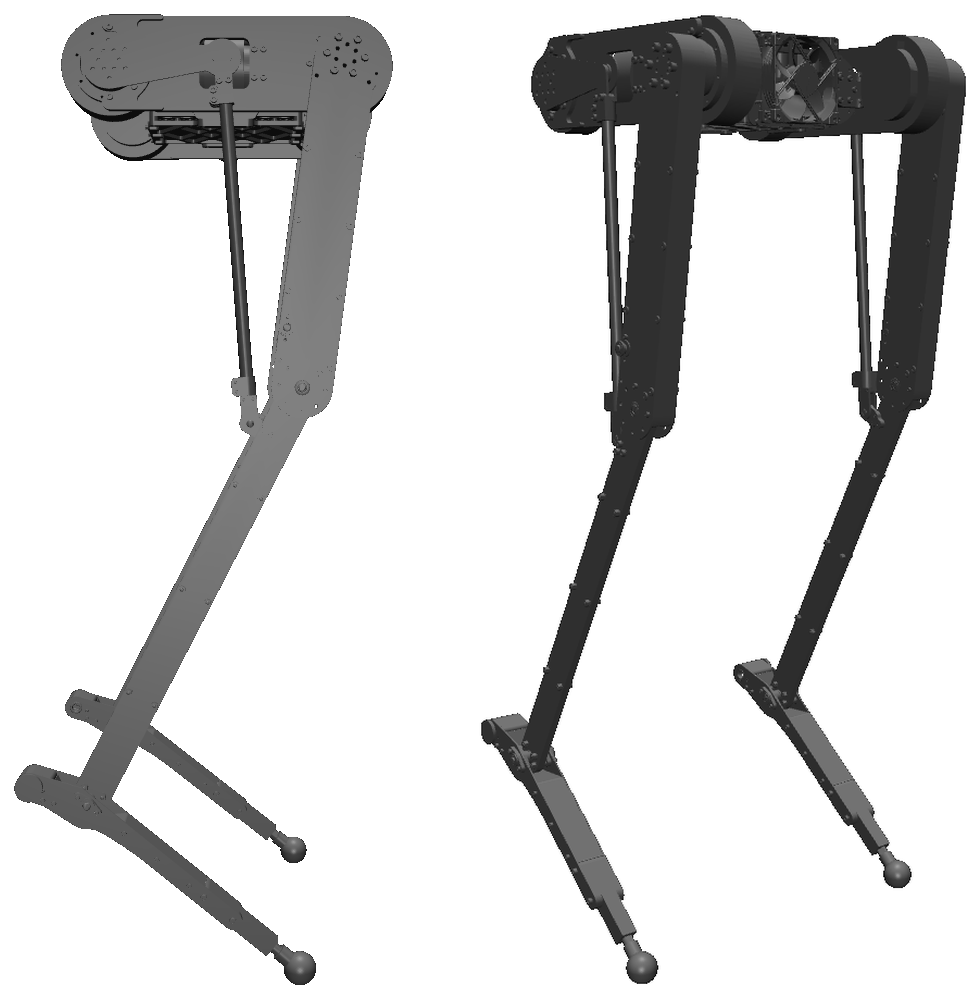
\includegraphics[width=\linewidth]{Figures/fig_robot.png}
\end{minipage}\hfill
\begin{minipage}[c]{0.35\textwidth}
  \centering
  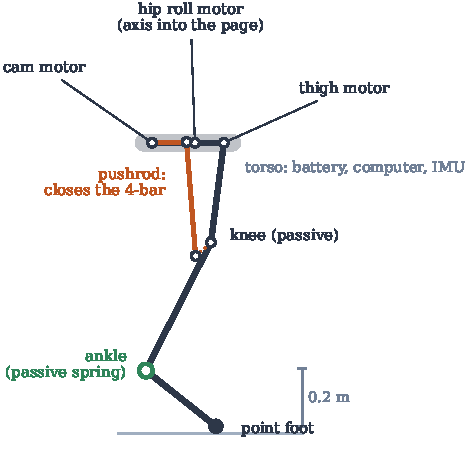
\includegraphics[width=\linewidth]{Figures/fig_leg.pdf}
\end{minipage}
\begin{minipage}[c]{0.22\textwidth}
  \centering
  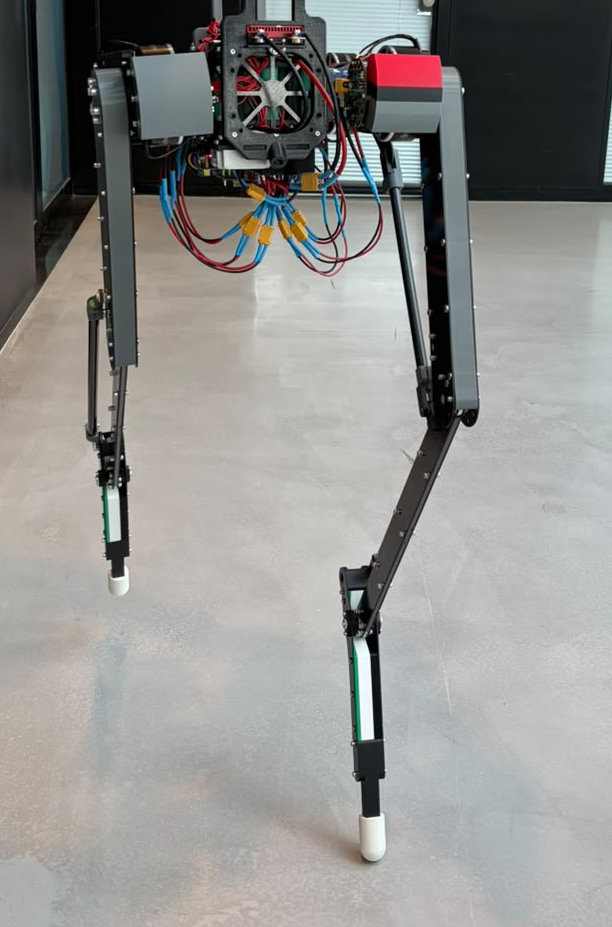
\includegraphics[width=\linewidth]{Figures/dash01-realife.jpg}
\end{minipage}
\caption{DASH-01, Simulated model and real-life picture.}
\label{fig:robot}
\end{figure}

\begin{table}[H]
\centering
\small
\setlength{\tabcolsep}{3.5pt}
\begin{minipage}[t]{0.55\textwidth}
\centering
\begin{tabular}{lcc}
\toprule
& \textbf{Hip roll} & \textbf{Cam, thigh} \\
\midrule
Part & AK60-39 & AKE90-8 \\
Reduction & 39:1 & 8:1 \\
Peak torque, datasheet & 72\,N$\cdot$m & 170\,N$\cdot$m \\
Peak torque, measured & 61.2\,N$\cdot$m & 144.5\,N$\cdot$m \\
Continuous torque & 24\,N$\cdot$m & 55\,N$\cdot$m \\
No-load speed & 10.3\,rad/s & 22.0\,rad/s \\
$K_t$ (N$\cdot$m/A) & 0.12 & 0.272 \\
$R$ ($\Omega$) & 0.60 & 0.164 \\
$K_m$ (N$\cdot$m/$\sqrt{\text{W}}$) & 0.15 & 0.674 \\
Reflected armature (kg$\cdot$m$^2$) & 0.046 & 0.0216 \\
Mass (kg) & 0.75 & 1.40 \\
Unit price (EUR) & 393 & 424 \\
\bottomrule
\end{tabular}
\end{minipage}\hfill
\begin{minipage}[t]{0.43\textwidth}
\centering
\begin{tabular}{lrr}
\toprule
\textbf{Segment} & \textbf{Mass} & \textbf{Count} \\
\midrule
Base & 5764\,g & 1 \\
Hip, with two motors & 3271\,g & 2 \\
Cam & 66\,g & 2 \\
Thigh & 483\,g & 2 \\
Push rod & 71\,g & 2 \\
Ankle spring assembly & 249\,g & 2 \\
Shin & 324\,g & 2 \\
Foot & 222\,g & 2 \\
\midrule
\textbf{Total} & \textbf{15\,136\,g} & \\
\bottomrule
\end{tabular}
\end{minipage}
\caption{The six CubeMars quasi-direct-drive actuators (left) and the weighed segment masses
(right). Measured peak torque is the datasheet figure scaled by the effective joint $K_t$ of
\cref{sec:inertia-validation}. $K_t$ and $R$ are line-to-line, and the motor figure of merit is
$K_m = K_t/\sqrt{R}$. }
\label{tab:motors}
\end{table}

Each leg carries three motors. Hip roll sits at the base, and a cam and a thigh axis drive the
sagittal plane. The knee is passive and follows through the 4-bar. The ankle is passive and follows
through a spring (not rendered). The spring was later measured to be roughly an order of magnitude too soft: at half body weight it deflects 26.6\,deg, which would drive the heel 11.9\,mm through the floor. The ankle was therefore locked in a neutral position with a carbon tube, and the simulation masses were updated to reflect the change.


\newpage 

\subsection{Selecting hardware}
\label{sec:hw-selection}

\subsubsection{Actuators choice}
\label{sec:hw-motor}

A database to select the actuator was assembled.
Major robotic actuator manufacturers' websites were scraped for datasheets and a large language model was used to parse each datasheet.
The database content was then manually checked to ensure the LLM produce the expected result.
The resulting database holds 140 entries across 11 suppliers, listed in \cref{tab:manufacturers}.

\begin{table}[htbp]
\centering
\begin{tabular}{lr}
\toprule
Manufacturer & Actuator count \\
\midrule
ZeroErr       & 32 \\
MyActuator    & 29 \\
CubeMars      & 22 \\
SteadyWin     & 21 \\
Maxon         & 12 \\
MAB Robotics  & 8  \\
RobStride     & 7  \\
HEBI Robotics & 6  \\
Soceboz       & 1  \\
RSL-ETH       & 1  \\
mjbots        & 1  \\
\midrule
Total         & 140 \\
\bottomrule
\end{tabular}
\caption{Actuator manufacturers represented in the database}
\label{tab:manufacturers}
\end{table}

\begin{figure}[H]
\centering
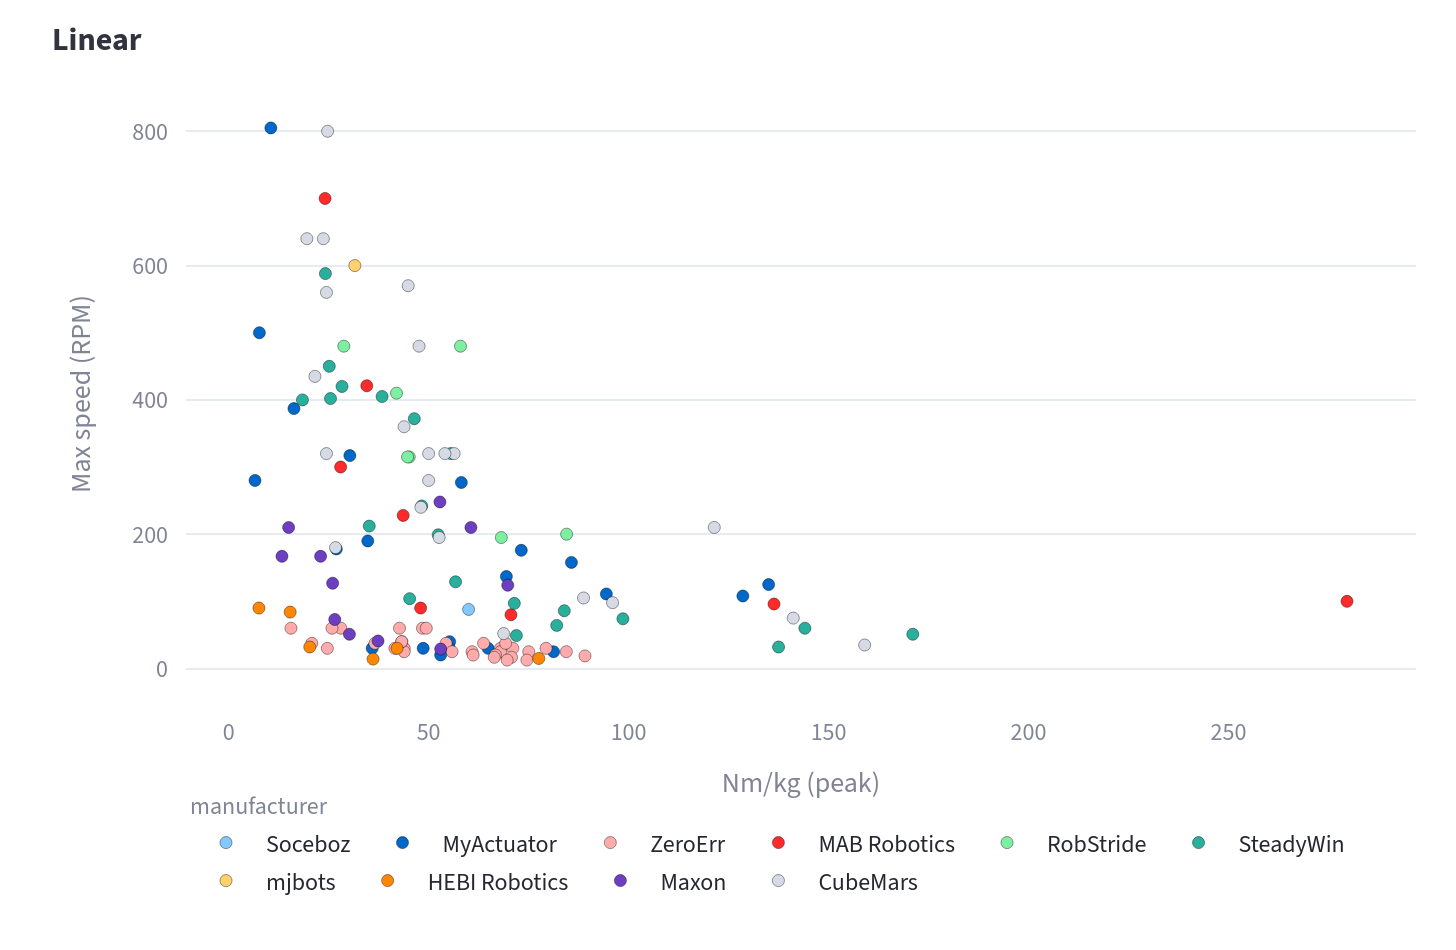
\includegraphics[width=1.05\textwidth]{Figures/ScreenshotActuatorMap.png}
\caption{Excerpt of the dashboard, showing the actuator database used to select the drive.}
\label{fig:motormap}
\end{figure}

The database was compiled into an interactive dashboard, \emph{motormap} \cite{morand2026motormap}, built from the \texttt{actuatorReview} code \cite{morand2026actuatorreview}.
The choice of the actuator itself is detailed in the master's thesis of M. Aebi \cite{aebi2025dash01}.
The final drive choice was the CubeMars AK60-39 for the hip roll and the AKE90-8 for the cam and thigh.
The AKE90-8 is rated for up to 72\,A peak, while the AK60-39 is rated for 17\,A peak.


\subsubsection{Compute, CAN bus and sensing}
\label{sec:hw-compute}

The following \Cref{tab:architecture} summarises the choice of the compute, sensing and network bus.
\begin{table}[H]
\centering
\small
\begin{tabular}{lp{9.3cm}}
\toprule
\multicolumn{2}{l}{\textbf{Compute}} \\
\midrule
Board & Raspberry Pi 3B, stock non-real-time Linux \\
Control loop & 200\,Hz \\
\addlinespace
\multicolumn{2}{l}{\textbf{Sensing}} \\
\midrule
IMU & ICM-20948, 10-axis, on a Waveshare Sense HAT\,(B) \\
IMU interface & I2C, $\pm4$\,g, $\pm1000$\,dps, 200\,Hz sampling \\
Analog input & 4-channel ADC on the same HAT \\
\addlinespace
\multicolumn{2}{l}{\textbf{Network bus}} \\
\midrule
Controller & \texttt{mcp251xfd} over SPI, dual-channel CAN HAT \\
Topology & two independent 1\,Mbit buses, one per leg \\
Measured load & 26\,\% of each of the two buses (polled at 200\,Hz) \\
\bottomrule
\end{tabular}
\caption{The robot's non-mechanical architecture: compute, sensing and the CAN network
bus.}
\label{tab:architecture}
\end{table}


\label{sec:compute-choice} The board is a \textbf{Raspberry Pi 3
Model B}, running stock non-real-time Linux. It was chosen over the laboratory's usual BeagleBone
Black for its faster SSH sessions and its four cores, which let the control loop and the data
processing run side by side.
An \texttt{mcp251xfd} controller over SPI provides CAN as two independent 1\,Mbit buses, one per leg.
The Pi also hosts a WiFi access point and the web interface of \cref{sec:deploy}, through which most measurements in \cref{sec:plant-id} were taken.

\Cref{sec:plant-id-timing} presents the measured timing of the control loop and the CAN bus.

Aside from the motor encoders and current feedback, the only proprioceptive sensor is the IMU located on the base of the robot.
Contact sensors were considered and never fitted due to lack of time.
The IMU unit is an \textbf{ICM-20948} on a Waveshare Sense HAT\,(B), read over I2C. 


\subsubsection{Battery choice}
\label{sec:hw-battery}

A database of roughly 430 commercial cells was built on the same principle as the actuator database.
Since 48\,V is the highest pack voltage the selected drives accept, the database was filtered to cells usable in a 13S configuration.
The motor selection sets the current requirement. Assuming half of the six motors at peak torque simultaneously (two AKE90-8 and one AK60-39), the pack must deliver about 160\,A.
From these candidates, a 13S2P pack of EVE INR21700-50PL cells was selected, as the best compromise between energy density, power density and cost.

The pack can be monitored over Bluetooth and its limits configured there with the DALY BMS app.
A CAN interface is also available but was not used, due to lack of time.

The manufacturer states the internal resistance below 10\,m$\Omega$ per cell, which gives about 65\,m$\Omega$ for the 13S2P pack.
At the rated 360\,A peak, the voltage drop would reach 23\,V.
At the 160\,A working peak of the motor budget, the drop is about 10\,V, which the BMS low-voltage protection tolerates on a full charge.
Due to the lack of voltage feedback on the drives, this figure has not been verified on the real robot.
\begin{table}[htbp]
\centering
\small
\setlength{\tabcolsep}{4pt}
    \begin{tabular}{lp{3.5cm}}
        \toprule
        \textbf{Parameter} & \textbf{Specification} \\
        \midrule
        Cell & EVE INR21700-50PL, 5.0\,Ah \\
        Configuration & 13S2P \\
        Nominal voltage, capacity & 48.1\,V, 10\,Ah (468\,Wh) \\
        Continuous rating & 100\,A, cell-limited \\
        Peak current & 360\,A for 2\,s\\
        Mass (BMS, casing) & 3.5\,kg \\
        Power density (peak) & 4900\,W/kg \\
        Power density (cont.) & 1370\,W/kg \\
        Energy density & 133.7\,Wh/kg \\
        \bottomrule
    \end{tabular}
\caption{Specification of the selected 13S2P battery pack.}
\label{tab:battery-spec}
\end{table}

\begin{figure}[H]
\centering
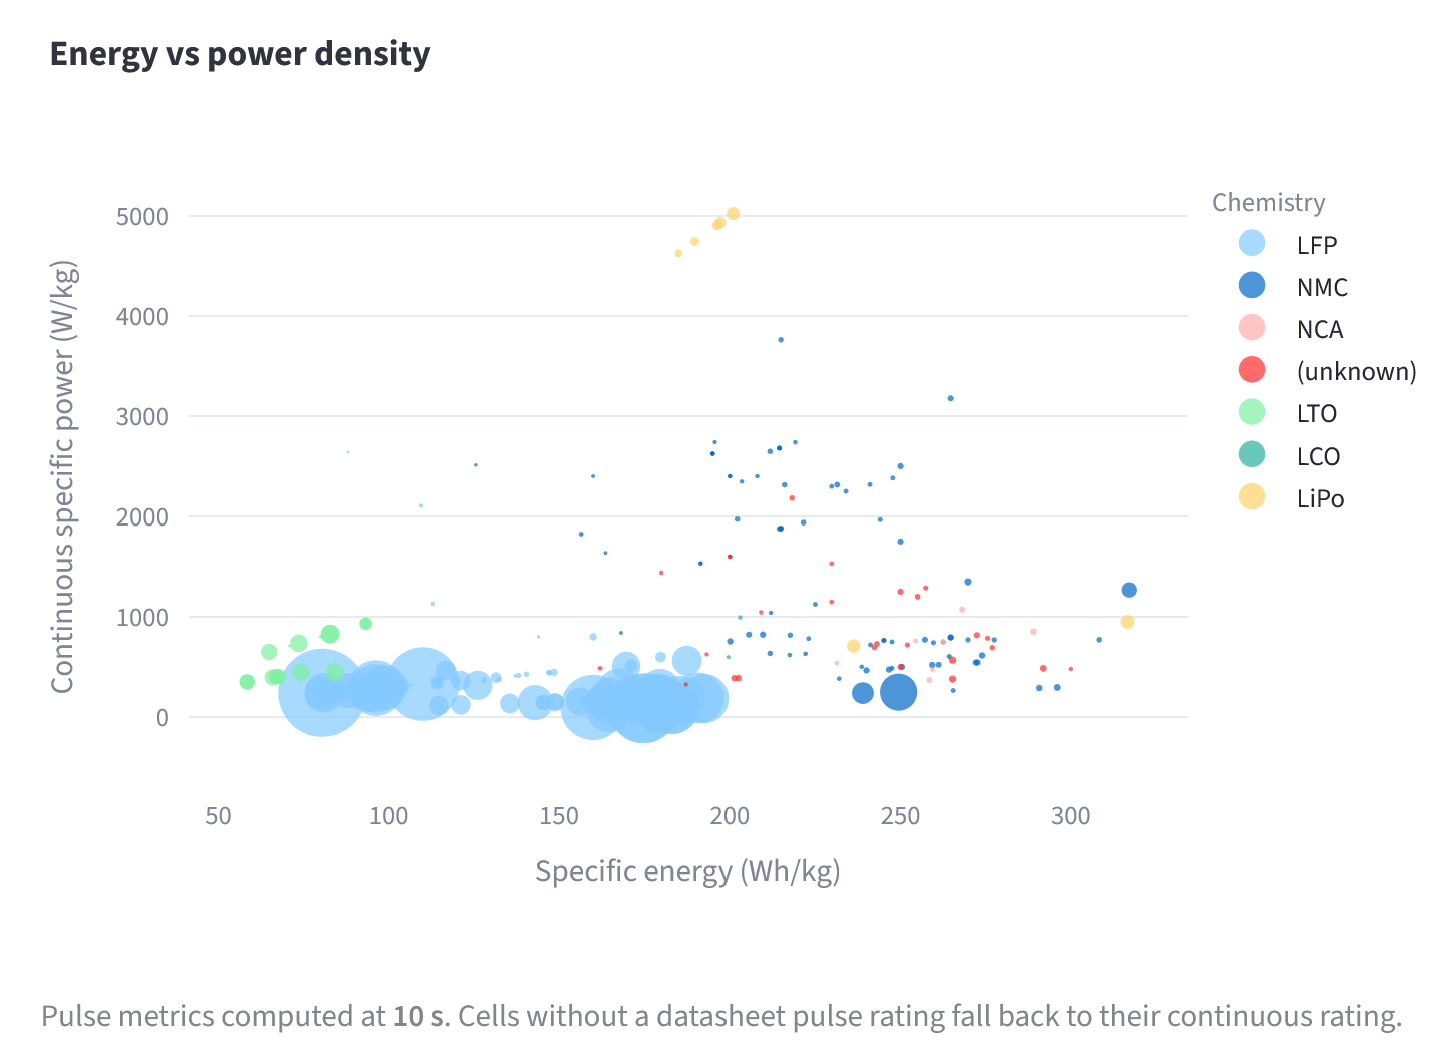
\includegraphics[width=1\textwidth]{Figures/cellDashboard.png}
\caption{Excerpt of the dashboard, showing the cell database used to select the pack.}
\label{fig:celldashboard}
\end{figure}

\newpage


\subsection{The digital twin}
\label{sec:twin}
A simulation ready model was derived from the CAD data. The model is exported in two formats, URDF and MJCF.
The detailed procedure to export the model is described in the appendix (\cref{sec:app-pipeline}).
This took a lot of time and effort due to lack of experience and the poor documentation of the plugin used to export the model.
The final recipe consisted of exporting each segment of the robot as a STEP file with the origin at the joint (except for the base which was in its centre).
Care was taken to ensure the reference axes were aligned in a consistent manner across the segments.
The robot model was reassembled in Autodesk Fusion 360 and exported to URDF using the ACDC4Robot plugin~\cite{qiu2024describing}.
The kinematic loop was broken in the URDF and closed in the MJCF using an equality constraint between two sites, one on the pushrod and one on the shin.
This was necessary because URDF is a tree format and cannot express kinematic loops.

\subsection{Digital twin validation and plant identification}
\label{sec:plant-id}
The digital twin is validated against the real robot for the kinematic and dynamic properties.
The model is also refined with measured parameters that cannot be accurately estimated from the CAD model, to reduce the sim2real gap.

\subsubsection{Joint Limits validation}
\label{sec:sim-hygiene}

The cam and thigh joints close a passive 4-bar loop through the pushrod and knee. Their safe ranges
do not compose into two independent intervals: a per-joint minimum and maximum would allow poses
the mechanism cannot assemble. The safe envelope is instead derived directly in actuator space.
Each leg's three drives are held current-free and the leg is backdriven by hand through its full
travel, logging the raw actuator angles \cite{morand2026runningrobot}.

\Cref{fig:joint-limits-actuator} shows the result for both legs: a plain interval for hip roll, and
a two-dimensional band for the coupled (cam, thigh) pair. The demonstrated hip roll range spans
42.8\,deg to 126.1\,deg on the left leg and 66.5\,deg to 147.7\,deg on the right; both are eroded by
3\,deg for a safety margin and the eroded interval is stored as the hip roll limit. For the knee pair,
the recorded (cam, thigh) samples are rasterised onto a 1\,deg grid, dilated to close small sampling
gaps, then eroded by the same 3\,deg margin. The stored safe region covers 11.0\,\% of its own
bounding box on the left leg and 9.4\,\% on the right, confirming the band is far from rectangular.
The onboard safety layer checks every commanded pose against this grid before it reaches the drives
(\cref{sec:safety}).

\begin{figure}[H]
\centering
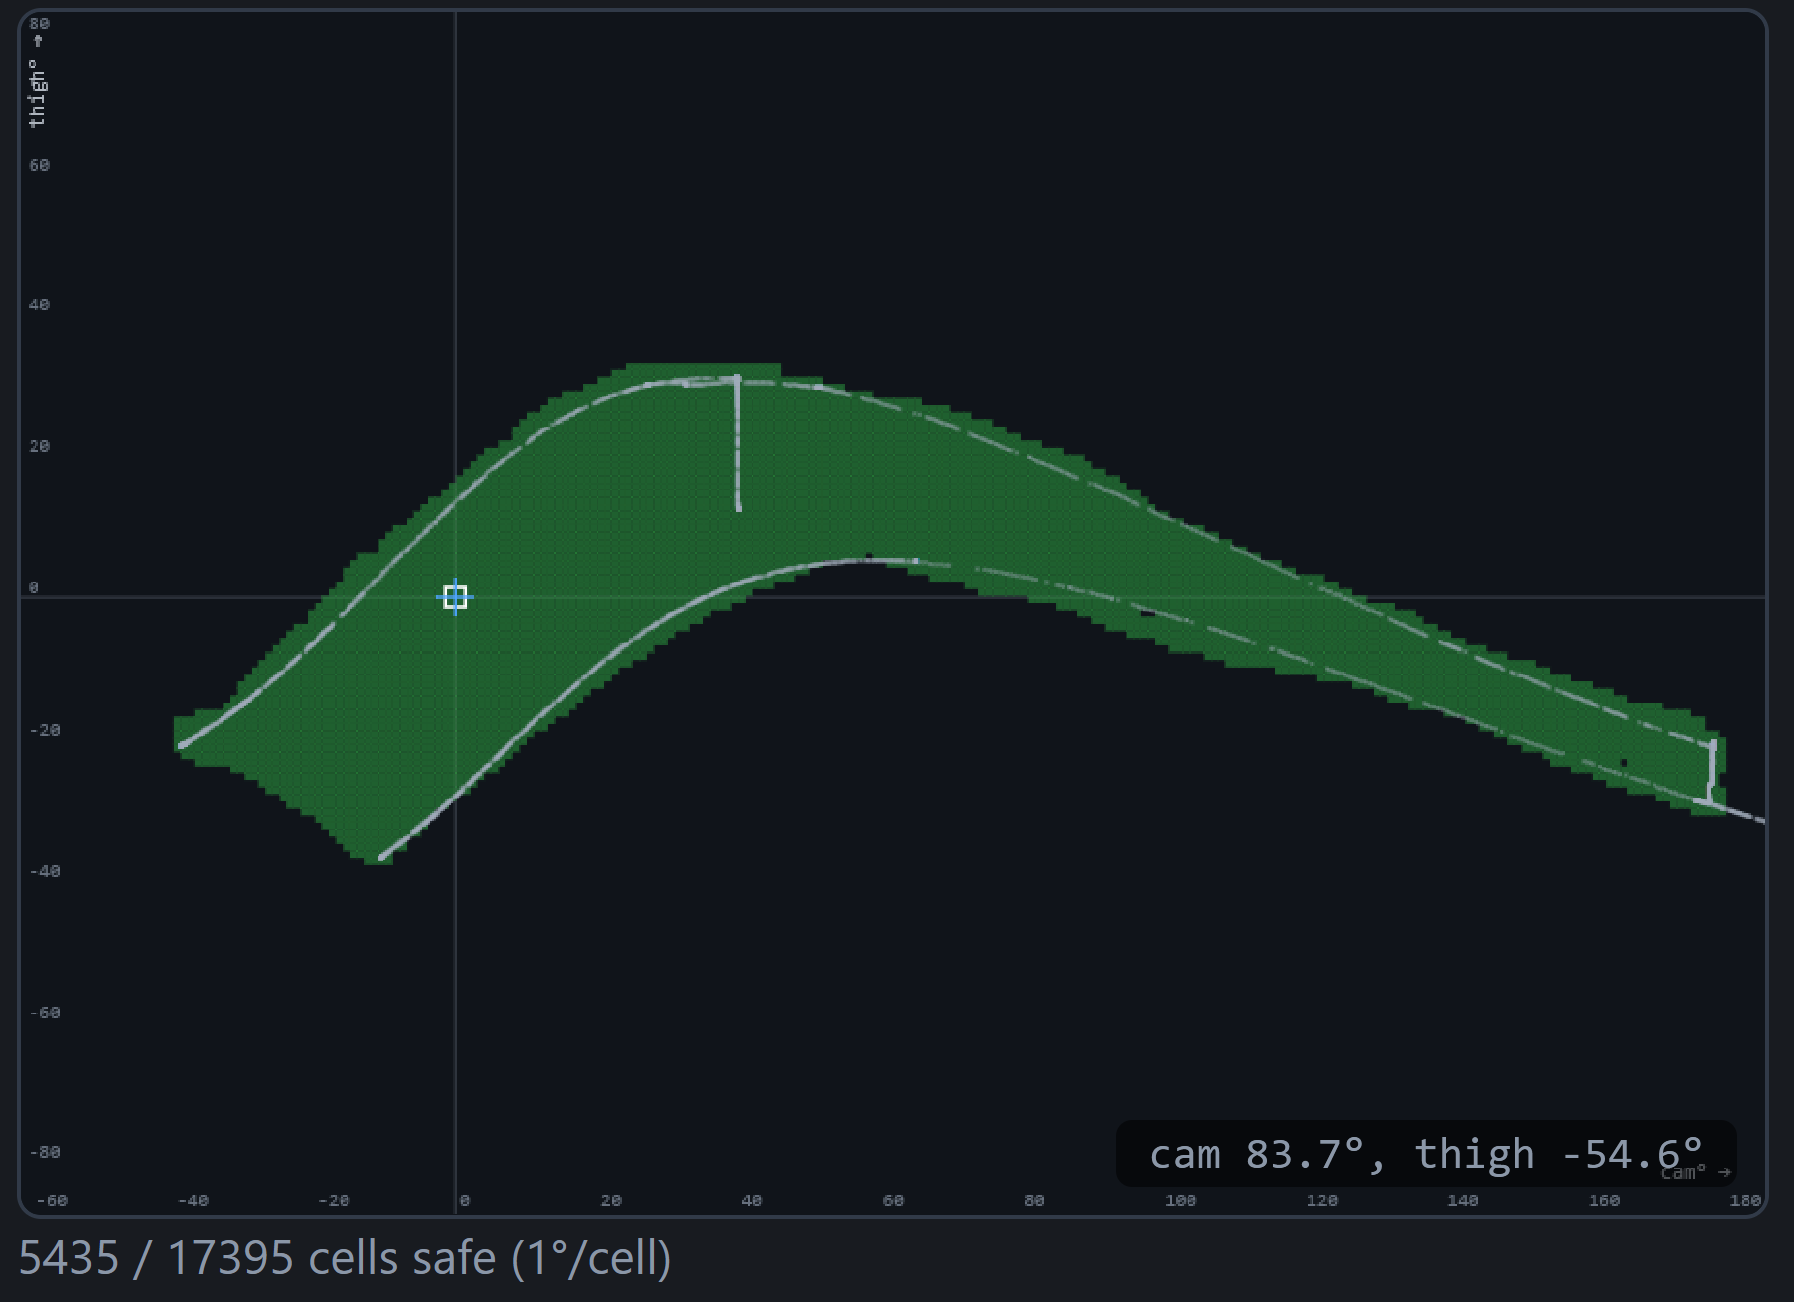
\includegraphics[width=0.95\linewidth]{Figures/fig_workspace_joint.png}
\caption{Joint-limit validation in actuator space: the coupled (cam, thigh) 4-bar band, backdriven by hand for each leg.
The green region is the safe envelope enforced by the onboard safety layer.}
\label{fig:joint-limits-actuator}
\end{figure}
\subsubsection{Inertia matrix validation}
\label{sec:inertia-validation}

The CAD export provides, for every body $b$, a mass $m_b$, a centre of mass $\mathbf r_{c,b}$ and an
inertia tensor $\mathbf I_b$, all expressed in the body frame. A wrong export transformation rotates
$\mathbf r_{c,b}$ and $\mathbf I_b$ without changing their magnitude, so the check below has to be
sensitive to the frame and to the magnitude separately.

Each actuated joint's torque constant $K_t$, effective inertia $I_{\mathrm{eff}}$ and friction
(viscous $b_v$, Coulomb $b_c$) are identified from two excitation profiles logged through the web
interface \cite{morand2026runningrobot}: a quasi-static sine sweep at 0.03\,Hz, which holds the
joint near equilibrium so gravity dominates the measured torque, and a 20\,s chirp from 0.05 to
0.6\,Hz, which excites the inertial term. Every joint obeys the single-DOF balance
\begin{equation}
K_t\,(i - i_0) = I_{\mathrm{eff}}\,\ddot q + b_v\,\dot q + b_c\,\mathrm{sgn}(\dot q) + \tau_g(\mathbf q),
\label{eq:joint-balance}
\end{equation}
where $i$ is the phase current, $i_0$ the drive's DC current offset and $\tau_g(\mathbf q)$ the
model's gravity torque at that joint, a function of the full configuration $\mathbf q$.

The gravity torque is computed from the inertial data by forward kinematics only, which stays
well-posed at the 4-bar singularity where inverse dynamics does not (\cref{sec:twin}). With
$\mathbf J_{c,b}(\mathbf q)$ the centre-of-mass Jacobian of body $b$ and $\mathbf g$ the gravity
vector, the gravity generalised force on all joints, actuated ($a$) and passive ($p$), is
\begin{equation}
\boldsymbol\tau_g(\mathbf q) = -\sum_b m_b\,\mathbf J_{c,b}^{\!\top}(\mathbf q)\,\mathbf g .
\label{eq:grav-torque}
\end{equation}
The closed loop couples the two sets. Linearising the loop-closure constraint,
$\mathbf J_a\,\delta\mathbf q_a + \mathbf J_p\,\delta\mathbf q_p = \mathbf 0$, gives the
passive-to-actuated map
\begin{equation}
\mathbf G = \frac{\partial \mathbf q_p}{\partial \mathbf q_a}
          = -\bigl(\mathbf J_p^{\!\top}\mathbf J_p + \lambda\mathbf 1\bigr)^{-1}\mathbf J_p^{\!\top}\mathbf J_a,
\qquad \lambda = 10^{-6},
\label{eq:loop-jacobian}
\end{equation}
damped so that it stays bounded at the singular poses, and by virtual work the gravity torque seen
by the actuated joints is the reduced-coordinate projection
\begin{equation}
\boldsymbol\tau_{g,a}^{\mathrm{red}} = \boldsymbol\tau_{g,a} + \mathbf G^{\!\top}\boldsymbol\tau_{g,p}.
\label{eq:grav-reduced}
\end{equation}
This is the $\tau_g$ used in \cref{eq:joint-balance} for the cam and thigh joints, which drive the
leg through the 4-bar; abduction is loop-independent.

Dividing \cref{eq:joint-balance} by $K_t$ makes it linear in the measured quantities. For the $N$
pooled samples of one joint, the regressor matrix $\boldsymbol\Phi \in \mathbb R^{N\times 5}$ and the
parameter vector $\boldsymbol\theta$ are
\begin{equation}
\boldsymbol\Phi_{k,:} = \begin{bmatrix} \ddot q_k & \dot q_k & \mathrm{sgn}(\dot q_k) & \tau_g(\mathbf q_k) & 1 \end{bmatrix},
\qquad
\boldsymbol\theta = \begin{bmatrix} I_{\mathrm{eff}}/K_t & b_v/K_t & b_c/K_t & 1/K_t & i_0 \end{bmatrix}^{\!\top},
\label{eq:regressor}
\end{equation}
and the estimate is the ordinary least-squares solution
\begin{equation}
\hat{\boldsymbol\theta} = \arg\min_{\boldsymbol\theta}\;\bigl\|\boldsymbol\Phi\,\boldsymbol\theta - \mathbf i\bigr\|_2^2
                        = \boldsymbol\Phi^{+}\,\mathbf i,
\label{eq:ls-fit}
\end{equation}
with $\mathbf i$ the stacked current samples. The quasi-static and chirp runs are simply
concatenated. The $\tau_g$ column varies with pose across the slow sweep and fixes
$K_t = 1/\hat\theta_4$; the $\ddot q$ column is large only during the chirp and fixes
$I_{\mathrm{eff}} = \hat\theta_1 K_t$; the friction terms follow from $\hat\theta_2$ and
$\hat\theta_3$. The intercept column is essential: over a short sweep $\tau_g$ is itself mostly
constant, so without it the drive's current offset lands in $\hat\theta_4$ and can flip the sign of
$K_t$. The inertia tensors enter through the second column: the tree mass matrix $\mathbf M(\mathbf q)$
built from the $\mathbf I_b$ gives the link contribution, and the rotor armature is the remainder
$J_{\mathrm{rot}} = I_{\mathrm{eff}} - M_{jj}(\bar{\mathbf q})$ at the median pose $\bar{\mathbf q}$.

A raw torque residual is hard to judge on its own, so it is converted into a mass-equivalent error,
\begin{equation}
\epsilon_m = \frac{\mathrm{RMS}\bigl(K_t(i_k - i_0) - \hat\tau_k\bigr)}{\mathrm{RMS}\bigl(\tau_g(\mathbf q_k)\bigr)},
\qquad
\hat\tau_k = I_{\mathrm{eff}}\,\ddot q_k + b_v\,\dot q_k + b_c\,\mathrm{sgn}(\dot q_k) + \tau_g(\mathbf q_k),
\label{eq:mass-error}
\end{equation}
the fraction of the gravity torque the model fails to explain, read as a relative error on the
segment masses. It is an upper bound, since a part of the residual is friction rather than gravity
torque. \Cref{fig:inertia-validation} reports the per-joint values. The relative error is large
because the segment masses are small, so their gravity torque sits close to the noise floor.

The check still serves its purpose. $K_t$ and the gravity model enter \cref{eq:joint-balance} only
through their product, so the fit alone cannot tell a scaled $K_t$ from a scaled mass; frame and
magnitude are therefore tested separately. The pose dependence of $\tau_g$ tests the frame of
$\mathbf r_{c,b}$, since a mis-rotated centre of mass changes the shape of the gravity curve and not
only its size. The recovered $K_t$ against the datasheet value tests the magnitude. Both confirm
that the inertial data are in the correct frame and of the correct magnitude, and that the gravity
trend is right. Since the CAD values are not random, a correct frame and magnitude imply the export
transformation is correct, and the CAD inertia data can be trusted. The bounded mass error
$\epsilon_m$ is reused as a domain-randomisation range in the RL training, to make the policy
robust to this uncertainty.

\begin{figure}[H]
\centering
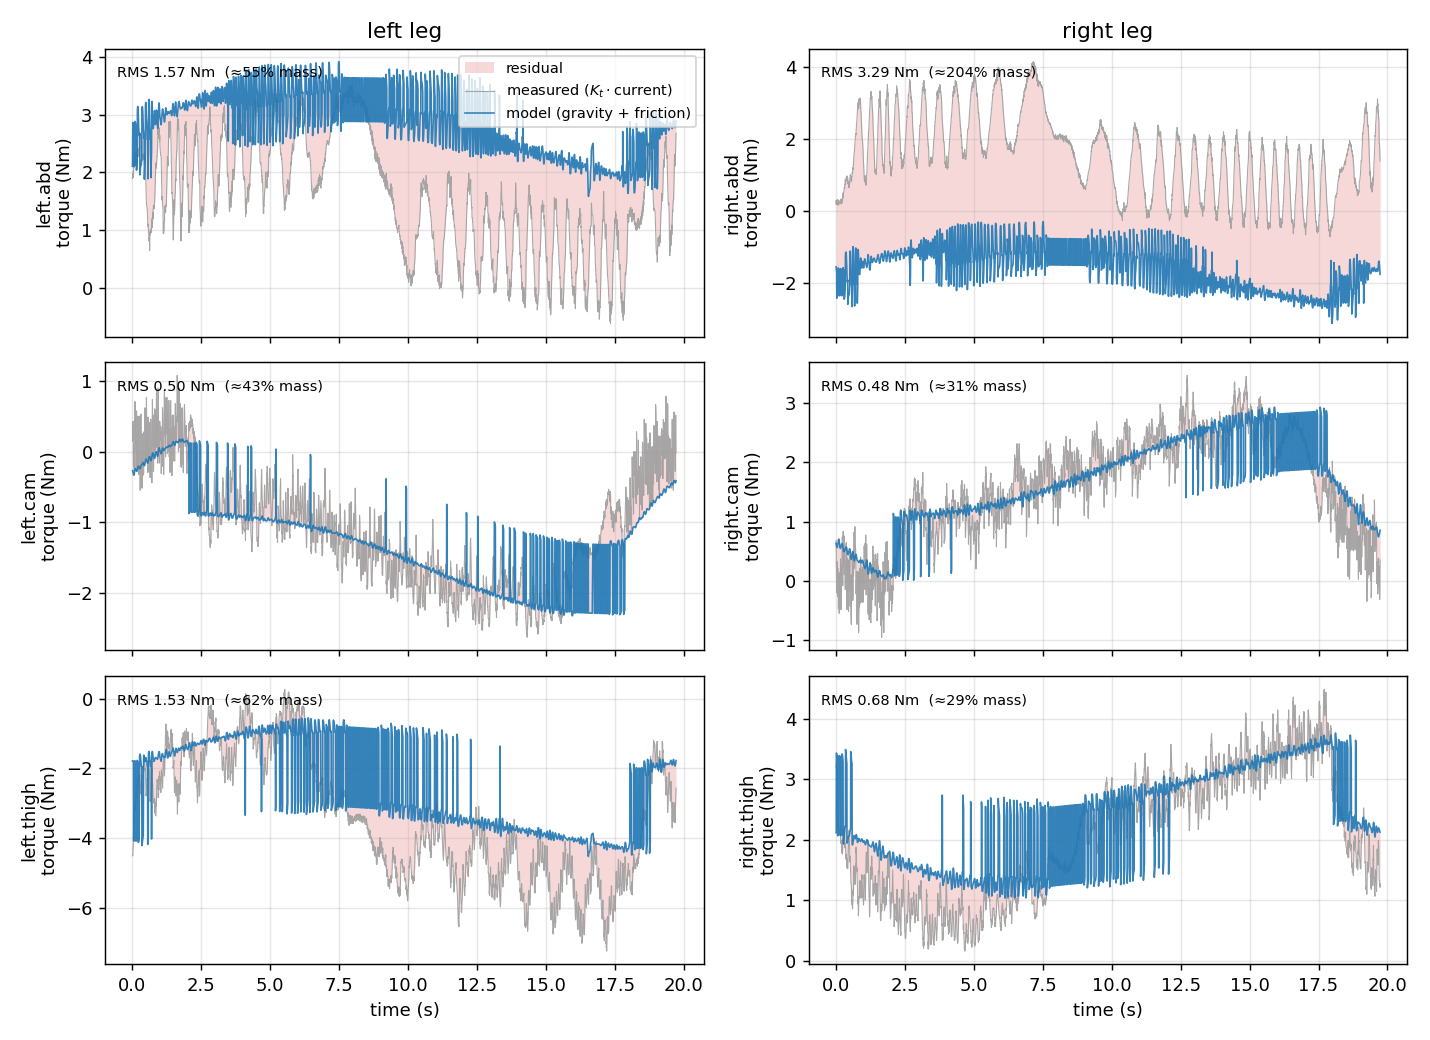
\includegraphics[width=0.9\linewidth]{Figures/inertiaValidationGravity.png}
\caption{Gravity-model validation on the slow (0.03\,Hz) quasi-static sweep: measured torque
($K_t$ times current) against the model's predicted torque (gravity plus friction), residual shaded,
per joint. The mass-equivalent error is the RMS residual divided by the RMS gravity torque. The fast
ripple is likely the P-only position loop's stick-slip response due to friction.}
\label{fig:inertia-validation}
\end{figure}


\subsubsection{CAN bus latency and load characterisation}
\label{sec:plant-id-timing}
The whole control loop was benchmarked on the robot with the web interface running.
These results were reused in the RL curriculum to make the policy robust to the timing jitter.

\begin{table}[htbp]
\centering
\small
\begin{tabular}{lrrrrr}
\toprule
\textbf{Rate} & \textbf{Mean period} & \textbf{Jitter (sd)} & \textbf{p99} & \textbf{Max} & \textbf{Budget used} \\
\midrule
50\,Hz  & 20.148\,ms & 2.151\,ms & 22.41\,ms & 49.29\,ms & 23\,\% \\
100\,Hz & 10.000\,ms & 0.251\,ms & 10.40\,ms & 12.28\,ms & 37\,\% \\
\textbf{200\,Hz} & \textbf{5.000\,ms} & \textbf{0.141\,ms} & \textbf{5.21\,ms} & 7.46\,ms & \textbf{50\,\%} \\
400\,Hz & 2.504\,ms & 0.193\,ms & 3.24\,ms & 5.13\,ms & 73\,\% \\
\bottomrule
\end{tabular}
\caption{Measured closed-loop timing on the robot's Raspberry Pi 3B, with the web interface competing for CPU.
One tick drains both CAN buses, runs a dummy inference of the policy and writes all the motor commands.}
\label{tab:loop-timing}
\end{table}

At 50\,Hz the mean period overshoots its 20\,ms target and the jitter is an order of magnitude above the faster rates.
The likely cause is the non-real-time scheduler, which wakes the loop late after the longer sleeps.
The dummy inference was later found to be too optimistic: the real policy requires the loop to run at 100\,Hz on the Pi 3B.


\subsubsection{IMU characterisation}
The base IMU was sampled at rest for 300\,s, configured at $\pm4$\,g and $\pm1000$\,dps, with a
50\,Hz internal low-pass and 200\,Hz sampling.
The measurement gives 1.8\,mg and 0.08\,dps RMS noise. The noise density is
218\,$\mu$g/$\sqrt{\text{Hz}}$ and 0.0096\,dps/$\sqrt{\text{Hz}}$. The gyro turn-on bias is
repeatable at $[1.03, 0.11, -0.53]$\,dps, and the in-run bias stability is 0.010--0.012\,dps.

\begin{figure}[H]
\centering
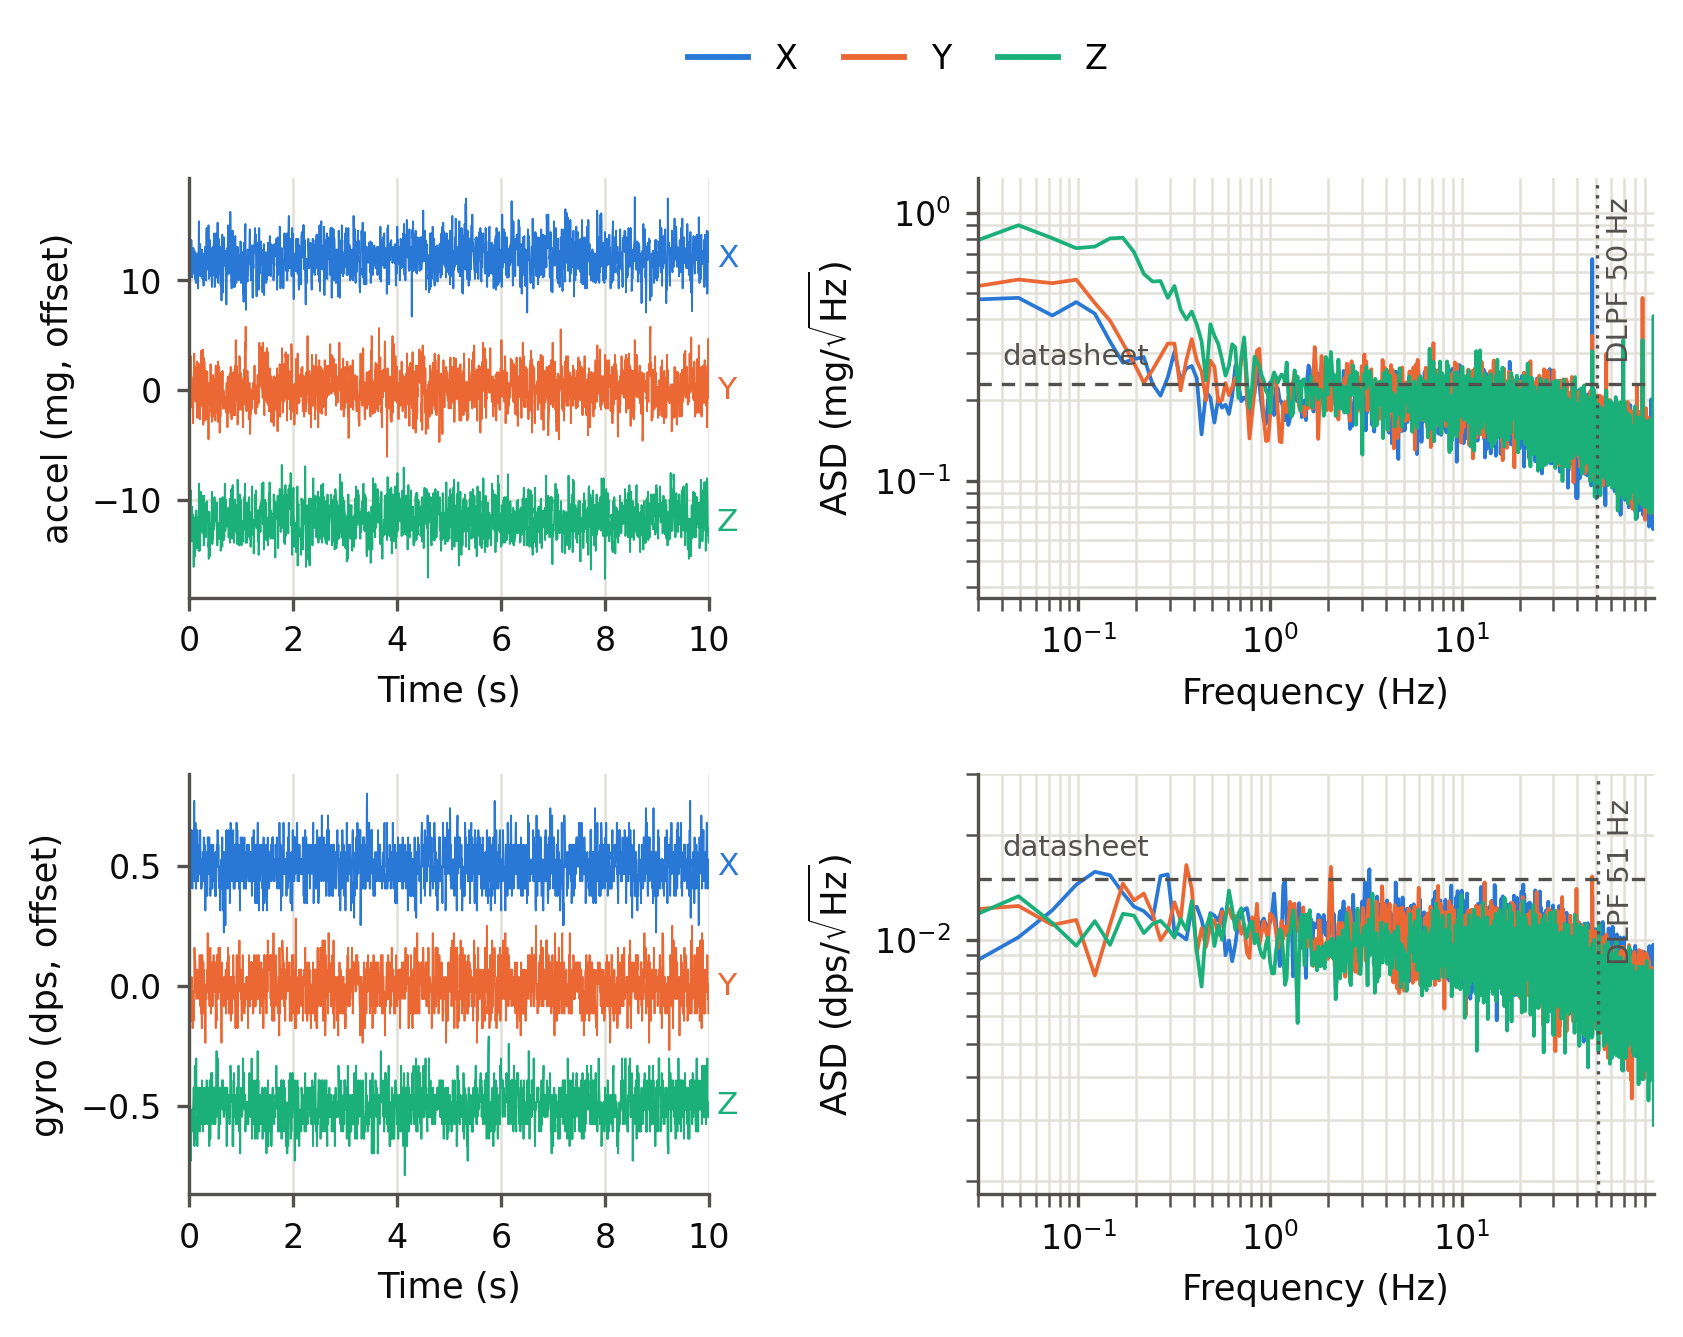
\includegraphics[width=0.9\linewidth]{Figures/fig_imu_noise.png}
\caption{Noise characterisation of the base IMU (ICM-20948), sampled at 200\,Hz for 300\,s at rest.}
\label{fig:imu-noise}
\end{figure}


\subsubsection{Actuator thermal characterisation}

The actuator thermal response was not measured due to lack of time. The thermal lumped model parameters were estimated roughly from the mass of the actuator but not used in the simulation.

\subsubsection{Battery characterisation}

The battery was not characterised due to lack of time; its behaviour was estimated from the datasheet internal resistance of the cell.
This is further complicated by the lack of voltage feedback on the drives, which prevents measuring the voltage drop under load.
In practice, this is not expected to be a problem: the drives are not used in torque control, so they can be expected to regulate the voltage drop without taking the RL policy out of its distribution.

\newpage 

\subsubsection{Actuator bandwidth characterisation}
\label{sec:plant-id-drive}

The AKE90-8's closed-loop position bandwidth was measured in both Servo and MIT mode, on the
thigh joints of both legs, with the legs attached but unloaded (robot homed on its stand). Both are position loops at the interface each mode is actually used through, so the two are
directly comparable. In Servo mode the command is a position set-point to the drive's internal
position loop. In MIT mode the drive runs its impedance law
\begin{equation}
\tau = k_p\,(p_{\mathrm{des}} - p) - k_d\,\dot p,
\qquad k_p = 200\ \mathrm{N\,m/rad},\quad k_d = 5\ \mathrm{N\,m\,s/rad},
\label{eq:mit-impedance}
\end{equation}
with the feed-forward velocity and torque held at zero. These are the deployed gains, the same
$\langle k_p, k_d\rangle$ actuator the policy is trained against in simulation
(\cref{sec:twin}). One extra run at $k_p = 500$ probes the stiffness dependence.

The excitation is a stepped sine, so that every frequency is measured in
steady state: 1 to 30\,Hz in 1\,Hz steps, at least 5\,s inside each frequency, with the frequency
switched at upward zero crossings so the command stays continuous. The command amplitude follows
\begin{equation}
A(f) = \min\!\Bigl(A_{\max},\ \frac{v_{\max}}{2\pi f}\Bigr),
\qquad A_{\max} = 0.044\ \mathrm{rad},\quad v_{\max} = 1\ \mathrm{rad/s},
\label{eq:bode-amplitude}
\end{equation}
constant position amplitude at low frequency and constant velocity amplitude above the corner, so
that neither excursion nor speed grows with frequency. Commands are streamed at 200\,Hz over CAN
and the drive's reported position, at the same rate and kernel time-stamped on reception, is the
measured output; its resolution is 0.1$^\circ$. A 200\,Hz watchdog aborts on drive error,
over-current, over-temperature or position leaving the safe window \cite{morand2026runningrobot}.

Per frequency, the first 1.2\,s after each switch are discarded and the reported position $p_k$
is projected by least squares onto the command's own sine and cosine, plus a mean and a linear
drift term,
\begin{equation}
p_k \approx a\,\sin\varphi_k + b\,\cos\varphi_k + c + d\,t_k,
\qquad
|H(f)| = \frac{\sqrt{a^2 + b^2}}{A(f)},\quad
\angle H(f) = \operatorname{atan2}(b, a),
\label{eq:bode-fit}
\end{equation}
where $\varphi_k$ is the command phase at sample $k$. Fitting on the exact command phase, instead of
an FFT bin, rejects the drift and the quantisation noise. Points whose response amplitude
falls below the position-feedback resolution, or whose residual exceeds 45\,\% of the response,
are masked since they are likely noise; the high-frequency Servo points end there by design. The
$-3$\,dB frequency is read by linear interpolation of the magnitude, and the loop delay from the
slope of the unwrapped phase above 4\,Hz,
$\tau_d = -\tfrac{1}{360^\circ}\,\mathrm{d}\angle H/\mathrm{d}f$.

\Cref{fig:actuator-bode} shows the results. Servo mode reaches $-3$\,dB at 1.9\,Hz on both thighs.
MIT mode reaches $-3$\,dB at 6.1 to 6.5\,Hz at the deployed gains, and 18\,Hz at $k_p = 500$ with
the same $k_d$: the corner scales with $k_p/k_d$, so the loop is damping-dominated. The phase
slope gives a delay of 11 to 13\,ms in MIT mode against 19 to 22\,ms in Servo mode.

\begin{figure}[H]
\centering
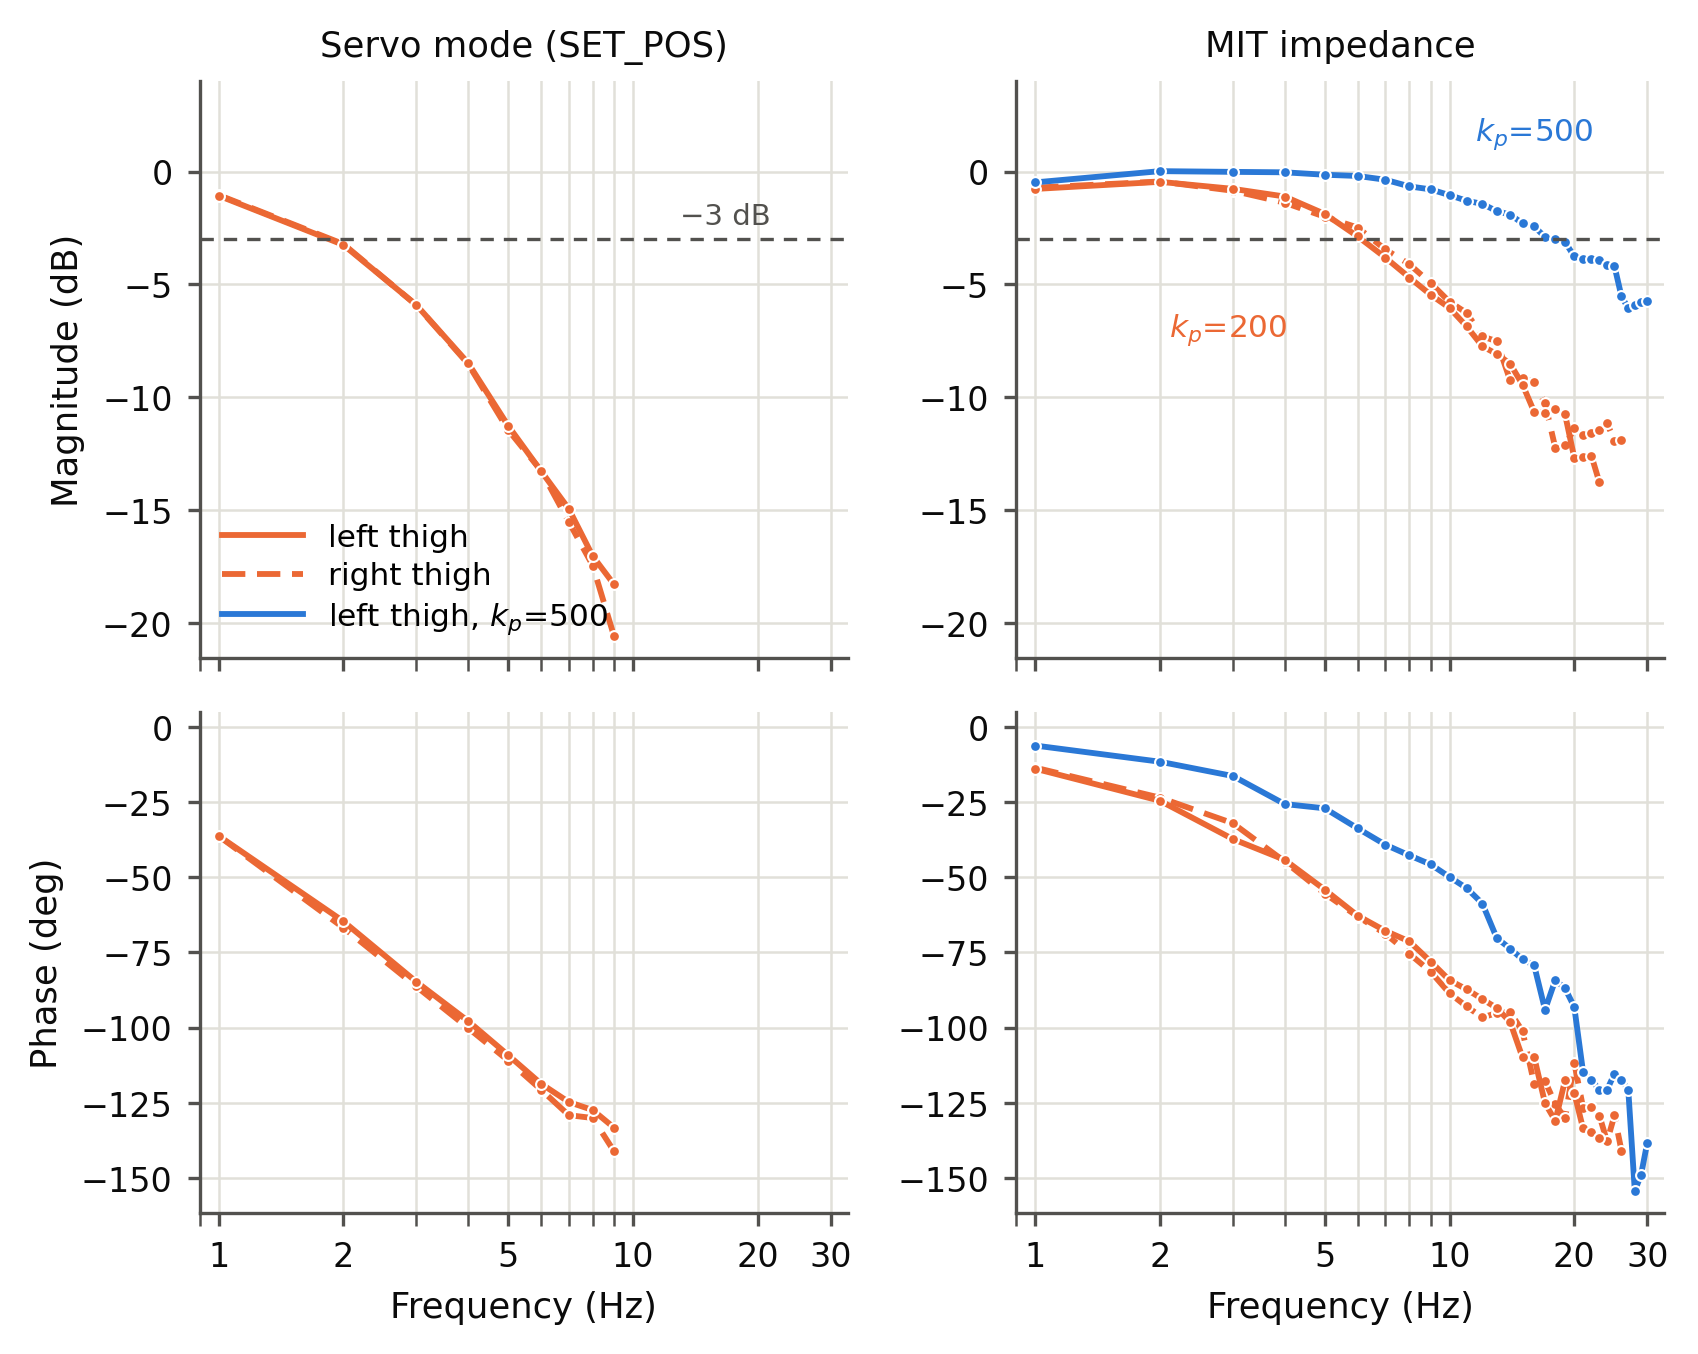
\includegraphics[width=0.75\linewidth]{Figures/actuator_bode.png}
\caption{Measured closed-loop position frequency response of the AKE90-8 thigh drives, both
legs, stepped-sine excitation 1--30\,Hz with legs attached and unloaded: Servo mode's internal
position loop against MIT mode's impedance loop at the deployed gains ($k_p = 200$, $k_d = 5$),
plus one MIT run at $k_p = 500$. Points below the 0.1$^\circ$ feedback resolution are masked.}
\label{fig:actuator-bode}
\end{figure}

\subsection{Deployment stack}
\label{sec:deploy}

The policies of \cref{sec:rl} have to run somewhere. To streamline the process and simplify the measurement of the plant parameters, a web interface was built on the robot.
A systemd entry starts the web interface at boot. The Raspberry Pi acts as a WiFi access point (SSID \texttt{runningmachine}, password \texttt{runningmachine}).
Once connected to the network, the web interface is reachable at \texttt{http://192.168.4.1:8080/}.

\subsubsection{Calibration sequence}
\label{sec:calibration}
The actuators do not hold their position when powered off, so a calibration sequence is needed to zero the joints.
The user needs to hold the robot in a known configuration and run the calibration sequence which registers the current joint position as zero.
The user then needs to move each joint in a specific direction and check that the angle increases (otherwise, the joint direction needs to be inverted by clicking a button in the web interface).
Once the robot is zeroed, the workspace can be registered by backdriving the robot and recording the joint position at the limit of the workspace.
The web UI then cleans the measurement to show the boundary and the user can draw / fill the safe workspace in the web interface.
This is used to limit the joint position in the safety layer.

The IMU is also calibrated in the web interface by holding the robot still and recording the bias of the accelerometer and gyroscope.
To ensure the axes are aligned, the user needs to move the robot around a given axis of the base and check that the correct axis is increasing.

\begin{figure}[H]
\centering
\begin{minipage}[t]{0.48\linewidth}
\centering
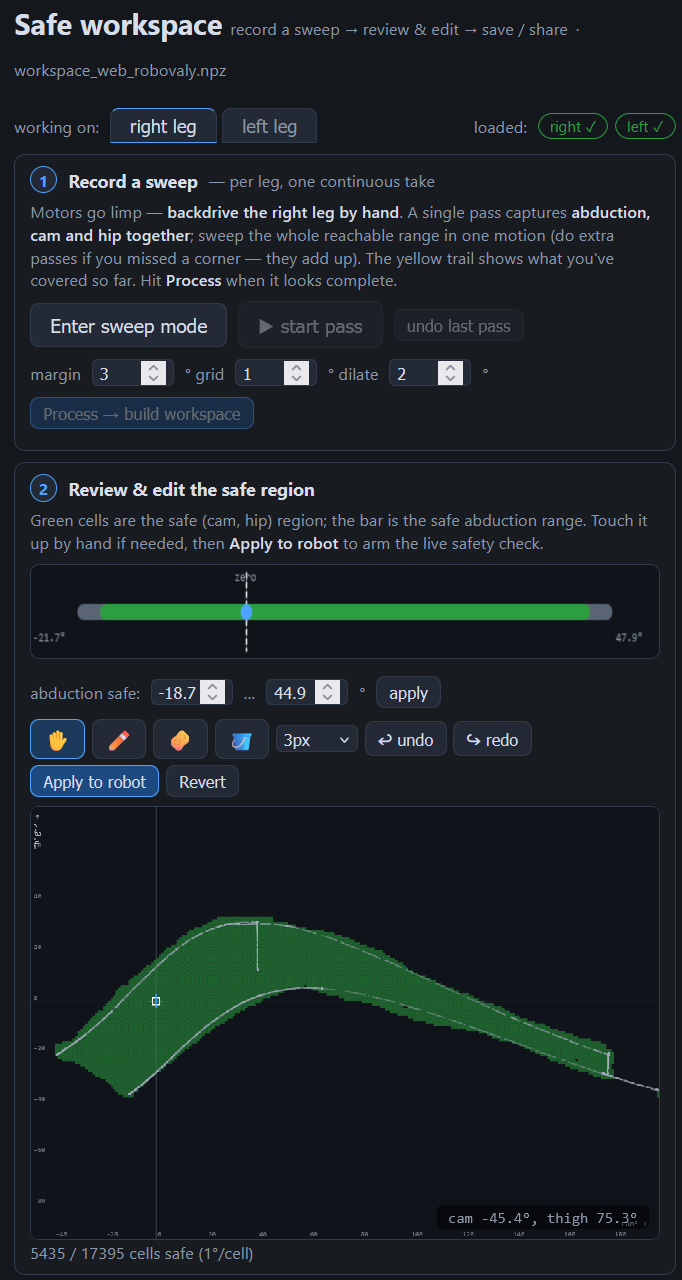
\includegraphics[width=\linewidth]{Figures/fig_WORKSPACEwidget.png}
\captionof{figure}{Workspace widget of the web interface, showing the backdriven joint envelope and the user-drawn safe workspace boundary.}
\label{fig:WORKSPACEwidget}
\end{minipage}\hfill
\begin{minipage}[t]{0.48\linewidth}
\centering
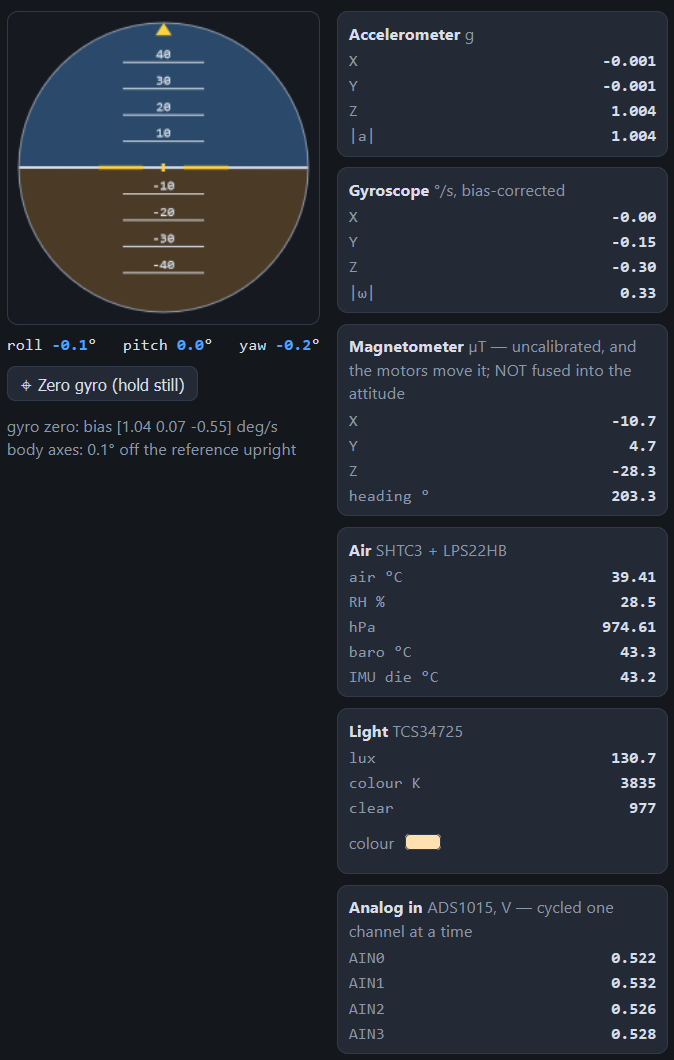
\includegraphics[width=\linewidth]{Figures/fig_IMUwidget.png}
\captionof{figure}{IMU widget of the web interface, used to record accelerometer and gyroscope bias and check axis alignment.}
\label{fig:IMUwidget}
\end{minipage}
\end{figure}


\subsubsection{The safety layer}
\label{sec:safety}

A safety layer was implemented to prevent the robot from exiting the safe operating envelope.
It limits the joint position, the joint speed and the joint torque. If a tracking error greater than a threshold is detected, the robot is stopped.
The user can also at any time stop the robot by clicking the E-STOP button in the web interface.
This safety layer was thoroughly tested in simulation and on the real robot by trying to make the robot exit the safe operating envelope and proved useful on a few occasions to prevent user error.
The safety layer also implements a black-box recorder that records the joint position, speed, torque and the IMU data at 200\,Hz. If a new failure mode is triggered, it will be possible to investigate it.

\subsubsection{Running widget}
\label{sec:hw-experiments}

From the web interface it is possible to both record a gait by backdriving the foot of the robot and then to play it back at a wanted frequency.
This is also where a policy can be selected and run on the robot.


\subsubsection{Measurement widget}
Three widgets carry the plant identification campaign of \cref{sec:plant-id}; \cref{fig:widget-measurement} shows them.
The \emph{thermal identification} widget deposits a known amount of electrical heat in one motor and records the case temperature, to fit a lumped thermal model.
The \emph{dynamic identification} widget excites one leg with workspace-checked position chirps and logs position, velocity and current at 200\,Hz. The recorded runs feed the fit of \cref{sec:inertia-validation}.
The \emph{limbs and inertia} widget stores the weighed segment masses and compares the CAD inertia tensors against the identified ones. The comparison uses the principal moments, which are frame-invariant, so wrong values are told apart from a wrong export frame.

\begin{figure}[H]
\centering
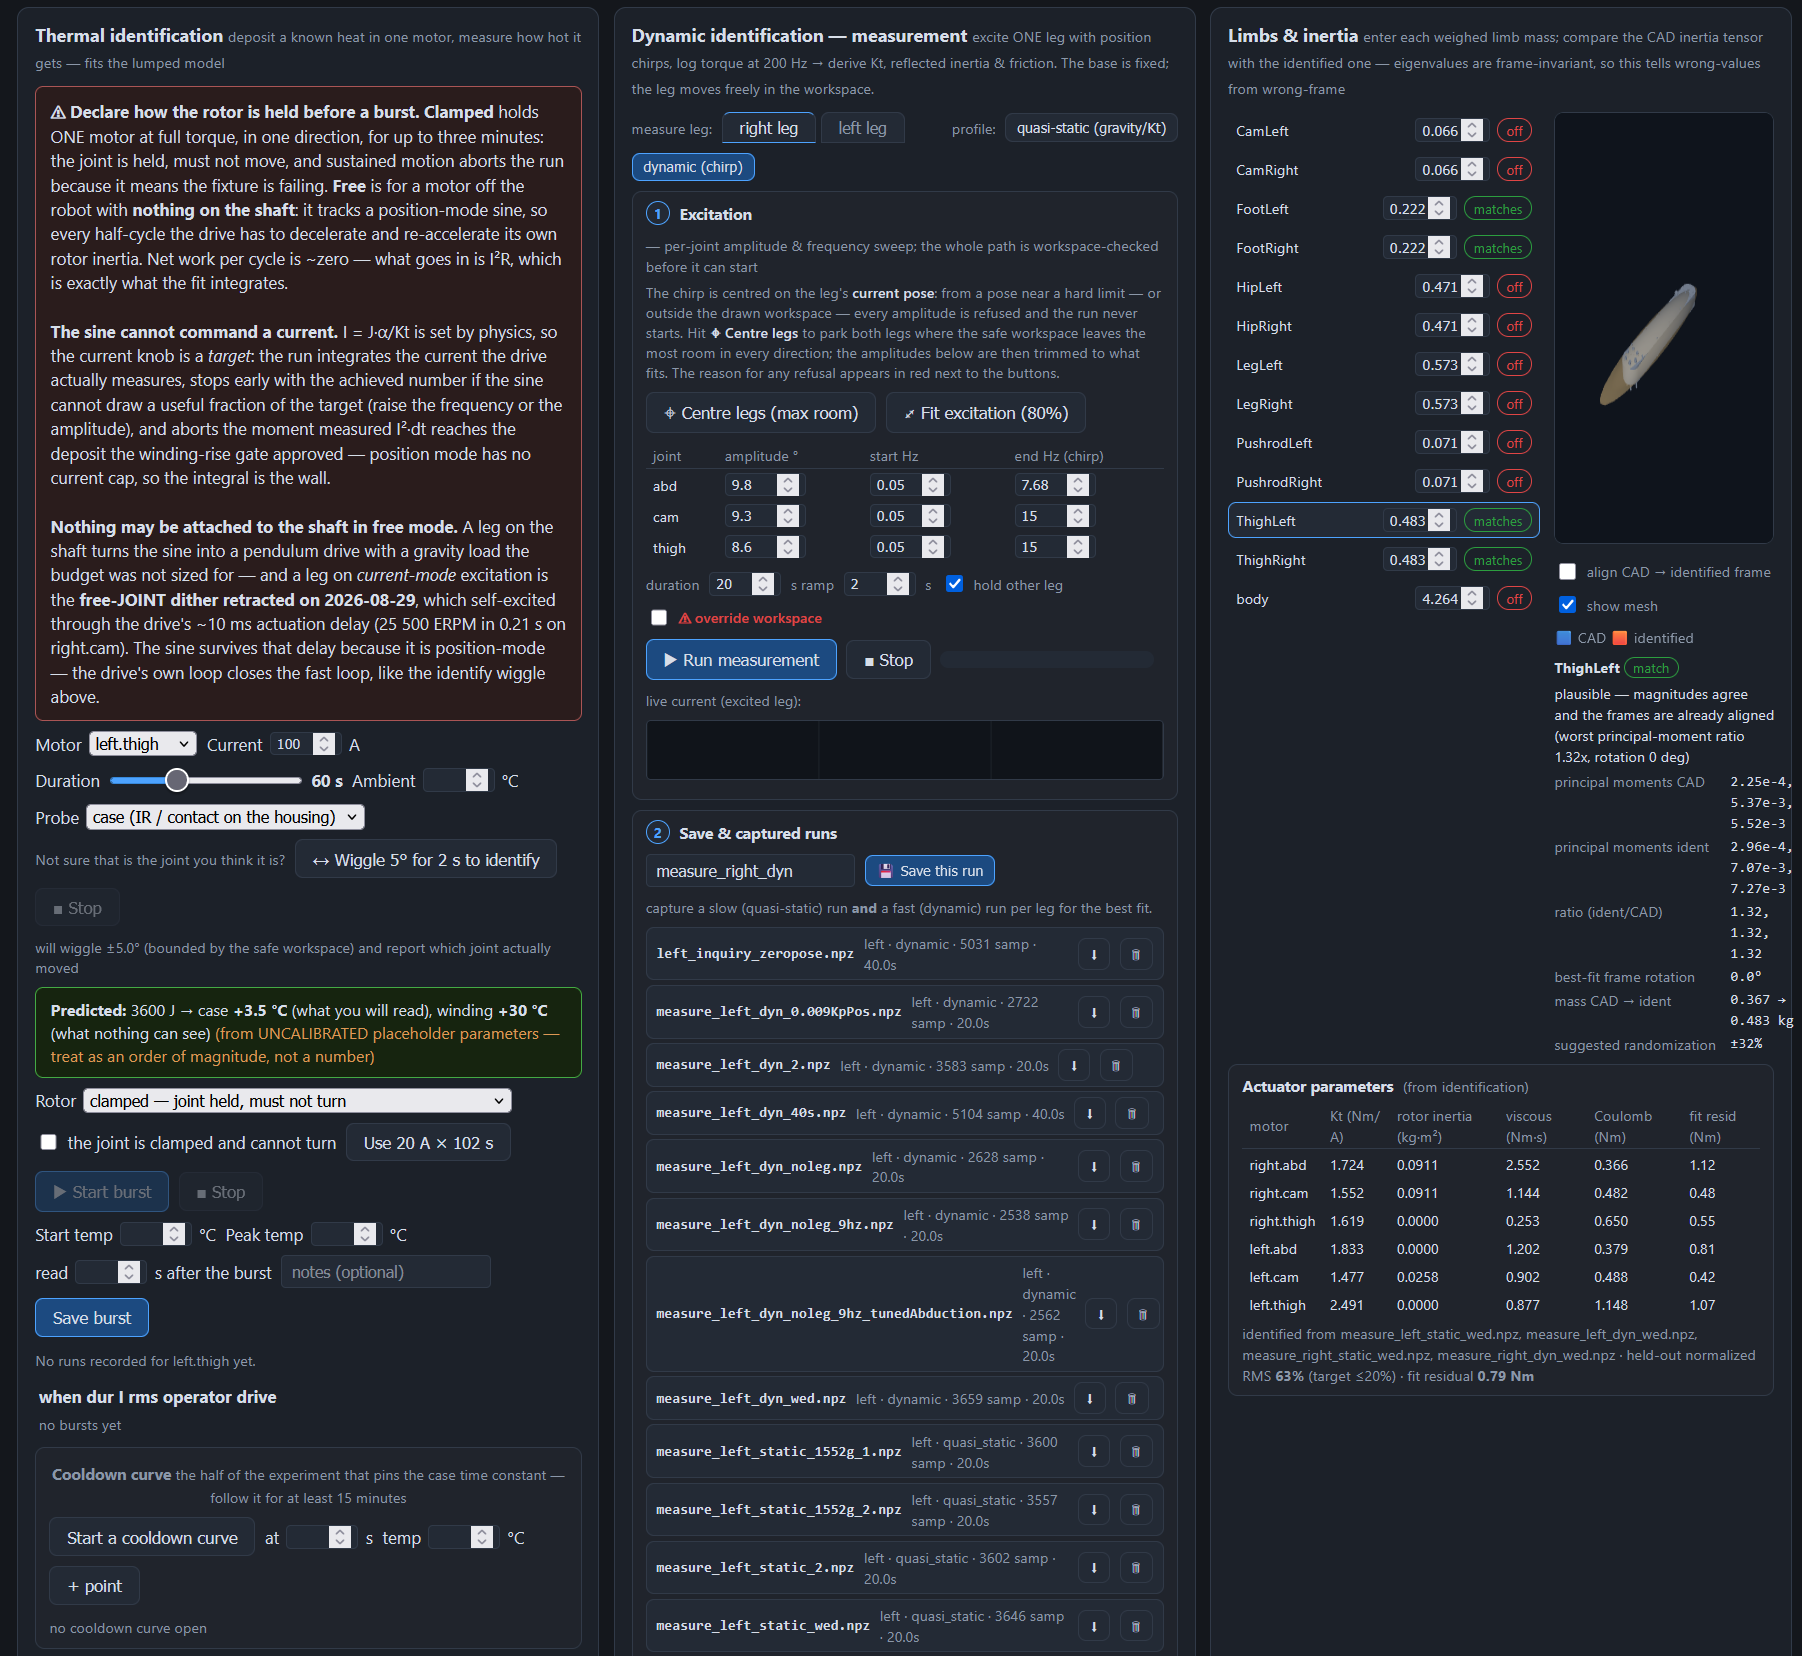
\includegraphics[width=1\linewidth]{Figures/MEASUREMENTSwidget.png}
\caption{The three widgets used to validate the robot parameters and limit the sim2real gap.}
\label{fig:widget-measurement}
\end{figure}


\newpage 

\subsection{Running speed ceiling estimation}
\label{sec:speed-ceiling}

The physical speed ceiling was established independently of reinforcement learning by applying progressively stricter physical constraints to the same robot model.
First,  the body was fixed and ground interaction removed with the leg free to move.
This was used to determine the maximum feasible fore-aft foot sweep over the empirically verified workspace.
The resulting speed was evaluated first from joint-speed limits alone, then with the measured torque-speed envelope and leg inertia, 
and finally with the measured actuator command latency.
This progressively reduced the theoretical ceiling from $14.5\,\mathrm{m/s}$ to $7.4\,\mathrm{m/s}$ and ultimately $6.55\,\mathrm{m/s}$, showing that actuator torque and leg inertia are the dominant limitations.
The result is an optimistic upper bound because the leg carries no body load and balance and contact constraints are ignored.

A second analysis extends the bound to gaits involving a flight phase, where the rail argument no longer applies because ballistic flight can increase stride length.
The maximum speed was instead constrained using an impulse balance: the available vertical foot force, obtained from the leg's force capability, was combined with the minimum time required to execute a stroke.
As speed increases, stance duration decreases while the leg's minimum cycling period remains finite, eventually leaving insufficient stance impulse to support the robot's weight.
This gives a slightly lower upper bound of approximately $6.2\,\mathrm{m/s}$.
Both analyses agree on a ceiling of about 6\,m/s, and this rounded figure is the bound quoted in the rest of the document.
For the details of the simulation, refer to the code itself.\cite{morand2026runningrobot}

\begin{table}[H]
\centering
\small
\begin{tabular}{lrrl}
\toprule
\textbf{Model} & \textbf{Bound} & \textbf{Cost} & \textbf{Binding mechanism} \\
\midrule
Kinematic (no-load speed only)        & 14.5\,m/s  & --      & joint speed through path Jacobian \\
+ torque--speed envelope, inertia     & 7.4\,m/s   & $-49$\,\% & stroke reversals, torque at speed \\
+ 7\,ms MIT-mode latency              & \textbf{6.55\,m/s} & $-12$\,\% & delay caps usable stiffness \\
\midrule
Flight-phase closure (any gait)       & \textbf{6.2\,m/s} & -- & vertical-impulse starvation \\
\bottomrule
\end{tabular}
\caption{The speed ceiling with refined modelling incorporating more realistic physical constraints.}
\label{tab:speed-ceiling}
\end{table}

\begin{figure}[H]
\centering
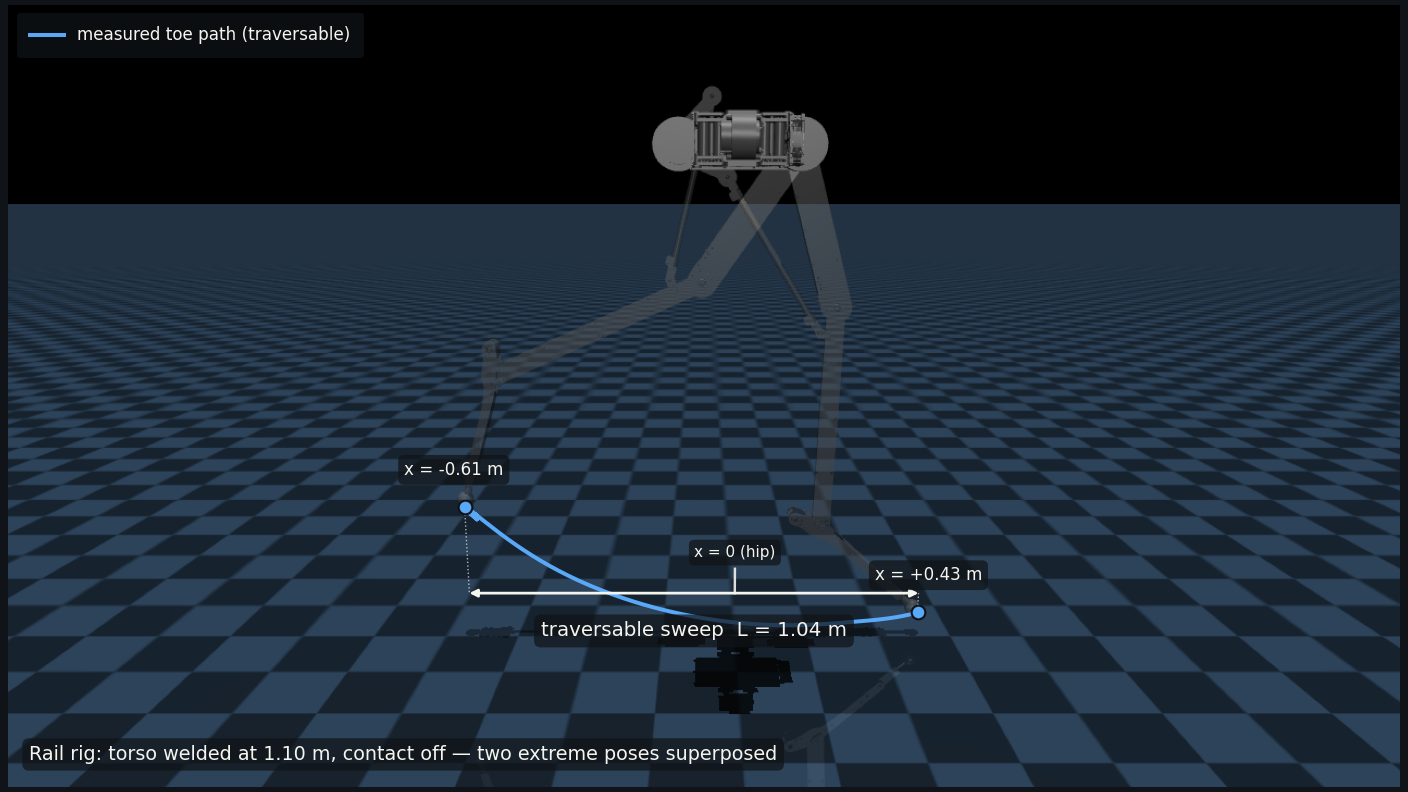
\includegraphics[width=0.85\linewidth]{Figures/rail_sweep_extent.png}
\caption{Workspace of the leg used to infer an optimistic upper bound on the running speed.}
\label{fig:speed-ceiling}
\end{figure}

\subsubsection{Static toe-force map}
\label{sec:plant-id-force}

The speed bound of \cref{sec:speed-ceiling} needs the force the leg can put on the
ground. The leg's static force capability over the measured workspace is therefore mapped.

The domain is the backdriven workspace of \cref{sec:sim-hygiene}. The toe
Jacobian comes from the model's closed-loop forward kinematics (\cref{sec:twin}),
differentiated over a 1\,deg grid. The joint torques are capped at the measured
144.5\,N$\cdot$m of \cref{tab:motors}. The maximum pure-vertical force $F_z$ and
pure-horizontal force $F_x$ at each pose then follow from $\tau = J^\top F$.
Vertical values are clipped at 3.5 body weights as near full extension the leg acts
as a strut, and the Jacobian alone would admit an arbitrary vertical force there.
Poses past the 4-bar's fold boundary are cut, since force there is not usable.

\Cref{fig:force-map} shows the result in body weights (15.14\,kg). The capability
is strongly anisotropic. At the standing pose, near 96\,\% of reach, the force
ellipse is about 19:1: the leg pushes hard straight down and weakly fore-aft,
which is suboptimal for propulsion. The vertical map feeds the impulse
bound of \cref{sec:speed-ceiling}, and the anisotropy makes the linkage
proportions a design lever that is presented in \cref{sec:discussion}.

\begin{figure}[H]
\centering
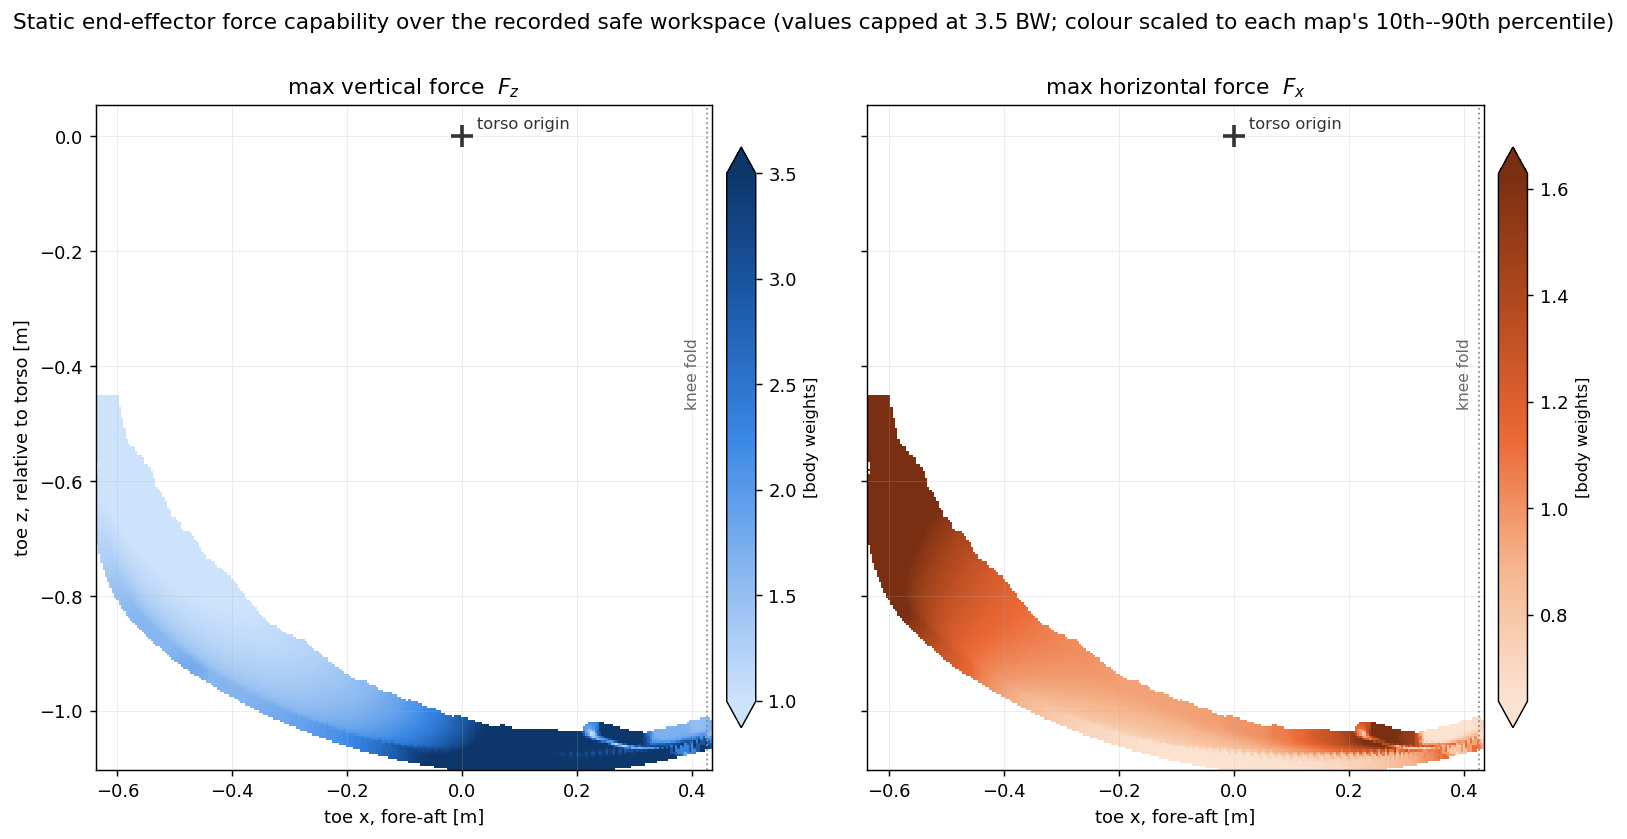
\includegraphics[width=1\linewidth]{Figures/fig_force_map.png}
\caption{Static toe-force capability over the measured workspace: maximum vertical force $F_z$
(left) and horizontal force $F_x$ (right), in body weights, clipped at 3.5\,BW. The vertical map
feeds the flight-phase impulse bound.}
\label{fig:force-map}
\end{figure}


\newpage 

\subsubsection{Sensitivity of the bound to the design parameters}
\label{sec:speed-sensitivity}

The rail model also gives the sensitivity of the bound to the design.
Four parameters were each scaled by $+50\,\%$ with everything else nominal: leg mass, rotor
inertia, deliverable peak torque and bus voltage (through the no-load speed).
Peak torque is the strongest lever: 50\,\% more raises the bound by about 1\,m/s in the worst case and 4\,m/s in the best one.
Leg mass is second: 50\,\% more lowers the bound by about 2\,m/s.
Rotor inertia is nearly flat, and 50\,\% more bus voltage gains nothing, because the bound does not
sit on the no-load-speed ceiling at this operating point.
Leg length was not simulated due to lack of time as it implies updating the URDF, but it is assumed that a longer leg would help increase the stride length.
The levers for a faster robot are therefore deliverable torque and leg mass.
Leg length is also likely a significant lever but its impact and direction are unknown.
\Cref{sec:discussion} ranks the mechanical changes that follow from them, and \cref{sec:rl} trains
its policies against the plant measured in this chapter.


\begin{figure}[H]
  \centering
  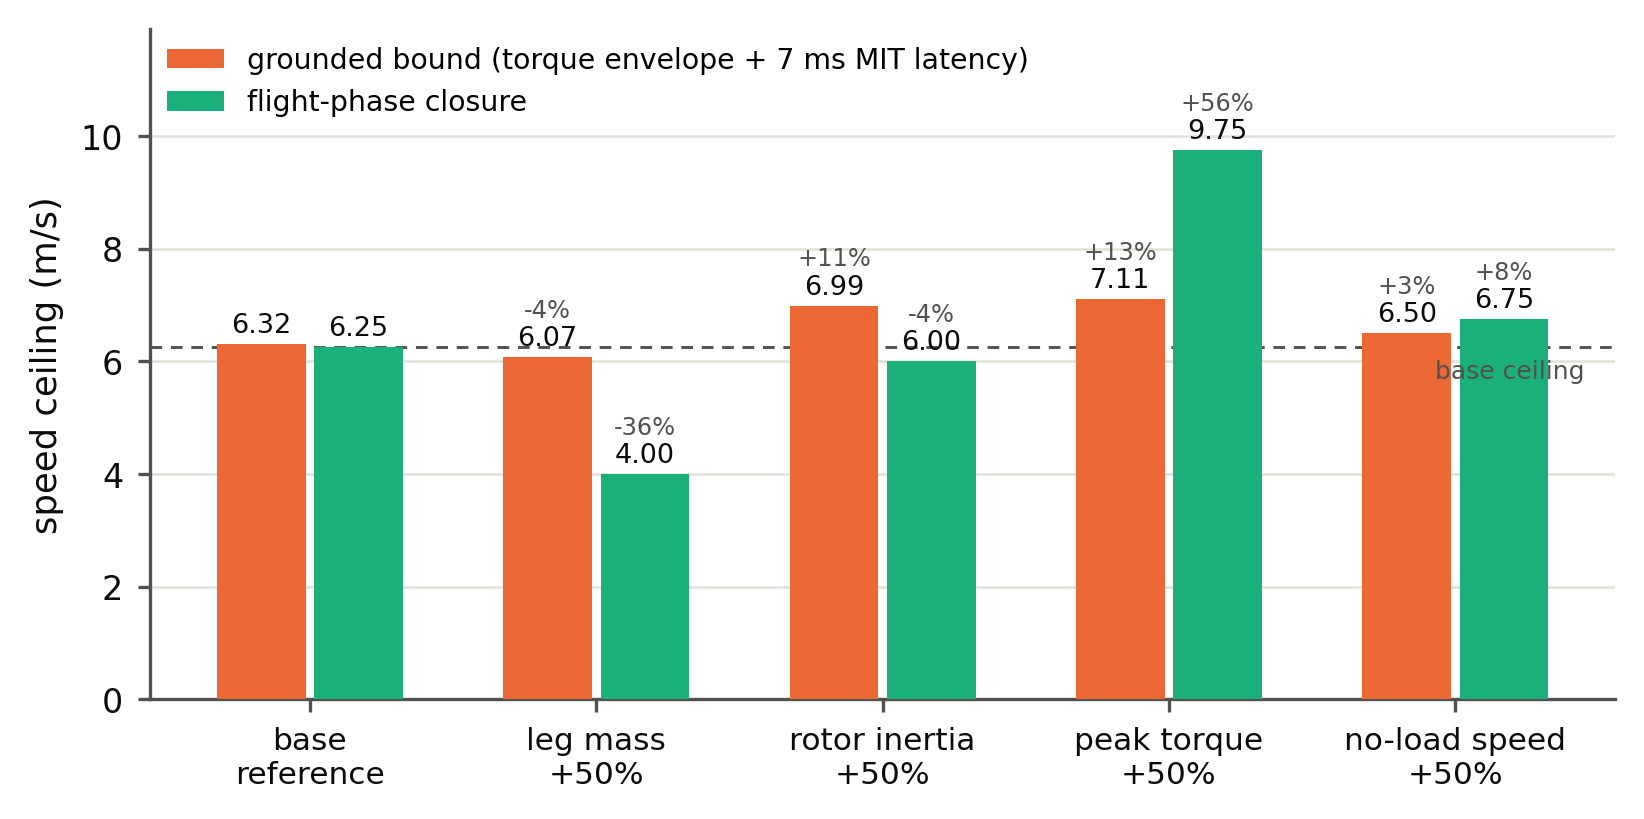
\includegraphics[width=1\textwidth]{Figures/bound_sensitivity_bars.png}
  \caption{Sensitivity of the speed-ceiling estimates to $+50\,\%$ design changes, one
  parameter at a time.}
  \label{fig:bound-sensitivity}
\end{figure}
\section{Results}

\subsection{Hardware selection}
show motor, battery pack, ...

\subsection{RL experiments}
show all the practical result we learned.



\section{Discussion}

\subsection{Sucesses}
What worked?
pipeline
modelling
standing
gait formulation

\subsection{Failures}
What did not work?
direct torque RL
fully autonomous running



\subsection{Lessons learned}
Simulation fidelity matters.
Action-space design matters.
Hardware integration dominates development time.
Progressive validation reduces debugging complexity.

\section{Discussion}
\label{sec:discussion}

This chapter measures the distance between the objective of \cref{sec:intro-objective} and the
results of \cref{sec:results}. It then answers the three hypotheses of \cref{sec:bg-gap}, and ranks
the changes that would close the gap. The ranking is the chapter's deliverable, and every entry
carries the measurement that ranks it.

\subsection{The distance to the objective}

The target was a bipedal 100\,m record pace near 4\,m/s. The measured mechanism sustains about
1.3\,m/s thermally, and bursts to about 2.7\,m/s (\cref{tab:speed-ceiling}). A 100\,m dash at
record pace is about 25\,s of continuous running against a continuous torque rating. The sustained
figure therefore decides the record, and the gap is a factor of three.

That gap is mechanical rather than algorithmic, and the evidence is a controlled comparison rather
than an inference. A 21-gain scripted controller with no learning in it hits the identical
pitch-balance wall at the identical time. The survival time equals the free-topple time of an
uncontrolled inverted pendulum, across a 5$\times$ change in the plant's time constant
(\cref{tab:freefall}). At that wall the set of stabilising action sequences is essentially empty,
so every controller drawn from it performs identically. No algorithm closes the gap on this plant.

\subsection{Verdict on the three hypotheses}

\textbf{H1, dimensionality reduction: supported.} The structural prior turned a non-converging
problem into a trainable one. The torque attempt is the control. It never converged, across an
unbroken sequence of reward-shaping attempts (\cref{sec:rl-torque}). The per-step position policy
converged only to standing, and skated (\cref{sec:rl-position}). The Fourier action space walked at
0.5\,m/s on its first trained policy, with no skating signature. The claim is scoped to this plant
and this sample budget. No arm was run at the $10^8$ to $10^9$ transitions per condition that the
published comparisons use.

\textbf{H2, control authority: partially supported, and the interesting half is untested.} Gait
morphology alone was not sufficient. Removing the per-step residual channel from the oscillator
generator produced stability without locomotion, at 15\,m of a 72\,m course (\cref{sec:cpg-ab}).
The reflex and residual channels were therefore necessary. The impedance level of the hypothesis,
phase-dependent $K_p(\varphi)$ and $K_d(\varphi)$, was designed and never run. The drive mode it
needs was never switched on the hardware (\cref{sec:rl-impedance}). H2 is answered for the residual
channel, and open for the impedance channel.

\textbf{H3, robustness across the sim-to-real boundary: untested on hardware.} No policy has run on
the robot. The closest available evidence is the descent onto the measured 0.8\,Hz drive. The
structured controller completed it, to an episode length of 4938 and three times its parent's score
(\cref{sec:sim2real-lineage}). That is a sim-to-sim result on a measured plant. No unconstrained arm
was run through the same descent for comparison, so it does not answer H3 as stated.

\subsection{Ranked levers for a successor robot}
\label{sec:future}

\begin{enumerate}[leftmargin=*]
  \item \textbf{Bus voltage before torque.} 87\,\% of feasible gaits are limited at the cam's
        peak-power corner (\cref{sec:speed-ceiling}). Over that population, speed scales with
        no-load speed and is insensitive to peak torque, and no-load speed is linear in bus
        voltage. The scope is the sweep as run, on the CAD plant. The cost is pack mass plus a
        drive rated for the higher voltage. A 60\,V variant of a drive already surveyed would have
        given 25\,\% for EUR\,220 (\cref{sec:hw-motor}).
  \item \textbf{Distal mass.} At $-0.93$\,(m/s)/kg it carries nine times the leverage of torso
        mass (\cref{tab:speed-ceiling}). A carbon shin, plus a proximally mounted spring on a
        tendon, recovers about 0.5\,m/s. The cost is a composite part and a tendon route to
        design. The carbon ankle already executed the cheap half of this, at $-209$\,g per shin
        (\cref{sec:ankle-build}).
  \item \textbf{Re-proportion or replace the 4-bar.} Only 0.20 to 0.35\,m of a 1.06\,m geometric
        span is usable. The standing pose sits at 96\,\% of reach, where the toe-force ellipse is
        19:1 anisotropic in the wrong direction (\cref{sec:hw-force-map}). Backward reach from the
        stance pose is 2.7\,cm against 31\,cm forward, which is why a backward fall can never be
        caught (\cref{sec:hw-experiments}). Target a flat transmission ratio over about 0.5\,m,
        with stance at about 85\,\% of reach. The cost is a linkage redesign. In the meantime,
        5\,cm of crouch buys most of the backward reach for 2\,N$\cdot$m out of 144.5.
  \item \textbf{Size the ankle for 3.5 body weights.} The passive ankle delivers a median of
        0.42\,BW over the running stance region, which is 8$\times$ short, and it fails in positive
        mechanical feedback (\cref{sec:hw-force-map}). The cost is either a stiffer passive element
        with correct preload, or a seventh and eighth motor. \Cref{sec:rl-pitch-wall} shows the
        passive route suffices in simulation, if the stiffness is achievable.
  \item \textbf{Cool the cam motor.} The demanded 167\,N$\cdot$m sits against a 55\,N$\cdot$m
        continuous rating, and the sustained figure is what decides a record. Cooling extends how
        long the peak stays available. The gain is unquantified, because winding temperature has
        never been logged at the measured duty cycle. \Cref{sec:speed-ceiling} records that as an
        open item. This is therefore a lever with a named test rather than a ranked result. The
        cost is added mass and an airflow path at the joint.
  \item \textbf{Treat torque-mode control as an architectural requirement from day one.} It was
        abandoned twice here, once on convergence and once on assumed deployability. The measured
        0.8\,Hz drive loop points back to it (\cref{sec:plant-id-drive}). Unlike the levers above,
        this one carries no number. In my view it is a design opinion rather than a ranked result.
\end{enumerate}

Two items sit outside the ranking, because they are measurement gaps rather than design changes.
Pack voltage sag is unobservable from the drives, and plausibly worth 30\,\% of joint speed at the
ten-second current tier (\cref{sec:hw-battery}). A voltmeter across the pack during a sprint
settles it. And the actuator's reference frame for reported current is undocumented, which puts an
unquantified risk on every measured torque figure (\cref{sec:hw-motor}). A clamp meter on a stalled
motor settles that one.

\subsection{Levers for this robot, in the order that unblocks the next}

\begin{enumerate}[leftmargin=*]
  \item \textbf{ONNX export and a Pi inference loop.} Everything else waits on it. The toy problem
        of \cref{sec:toy-problem} already demonstrated the path at one degree of freedom.
  \item \textbf{Current-mode control with the position PD closed on the Pi at 200\,Hz}, replacing
        the 0.8\,Hz drive loop that every measurement identifies as binding.
        \Cref{tab:loop-timing} shows the budget exists.
  \item \textbf{The carbon ankle strut}, already fitted, and the corresponding retrain on the
        rebuilt plant.
  \item \textbf{A from-scratch retrain with cadence pressure from step zero.} Every warm-started
        run stays trapped in the fast-stepping basin (\cref{sec:rl-cadence}).
  \item \textbf{The phase-dependent impedance experiment} of \cref{sec:rl-impedance}. Items 1 and 2
        make it possible, and it closes the open half of H2.
\end{enumerate}

\subsection{Method-level lessons}

The lessons below are the ones that survive a plant change, by the test of \cref{tab:survives}.

\textbf{Optimisers exploit objectives, and neural networks are not the culprit.} The policy gamed
the reward by skating, penetrating the floor, shuttling and committing suicide by penalty. The
scripted baseline's coordinate-descent tuner gamed its own objective identically. It drove at
1.6\,m/s against a 0.3\,m/s command, to farm a distance term (\cref{sec:scripted-baseline}). On
those two cases, in my view every objective needs adversarial review before its optimiser gets it.

\textbf{The margin advantage of learning rests on three premises, and none was paid in full here.}
The first is an exact plant, which this was not, since every parameter moved. The second is a
reward pricing distance from the failure boundary, which this did not, since it priced survival and
distance. The third is an asymptotic budget, which 600\,M steps per milestone is not. The
generalisable diagnostic is that seed variance is the margin measurement. A figure of
20.3\,$\pm$\,21.6\,s against 5 of 5 at the cap is bimodality rather than a worse mean, and a curve
plotting the mean will not show it.

\textbf{A gait prior reads on two axes, and the useful question is which kind rather than how
much.} A shape prior fixes the trajectory and exposes its timing, so tuning does not enlarge the
reachable set. It is therefore safe only when the morphology has a natural template. A structural
prior constrains the class and leaves the member free. DASH-01 separates the two, because its cam
turned out to be a full crank with no biological analogue. The evidence that the wider space was
genuinely used is the cadence agreement between the learned optimum and the independent physics
sweep, both at about 12.4\,steps/s (\cref{sec:speed-ceiling}). In my view the two-axis reading is a
way of comparing systems usually filed under one label, rather than a measurement.

\textbf{Every assumed parameter measured later moved pessimistically.} Mass by $+18\,\%$, torque by
$-15\,\%$, drive bandwidth by $-16\times$, plus friction and the ankle. Measure before training.
And when a measurement lands, apply it as \emph{the} plant rather than as an optional variant, or
the wrong default gets trained on (\cref{sec:plant-id}).

\textbf{Simulation results need the same scepticism as rewards.} Six artefacts each produced a
clean, converged, wrong result. They were soft joint limits, constraints inactive at settle,
frame-relative safety checks, a stale keyframe, a solver-version split between the development
machine and the cluster, and an actuator velocity cap that was never present. The last let a policy
balance at 23\,rad/s on a 22\,rad/s motor. Self-tests, smoke gates or measurement caught each one.

\textbf{Instrumentation found the ceilings, and cost something to build.} The measurement
instrument found the drive ceiling. The flight recorder found a daemon-killing crash and a dead bus
within its first hour (\cref{sec:deploy-blackbox}). The cost is that the measurement disturbed the
measured twice: once with the inertial sensor on a swaying rig, and once with the loop rate under
SSH load. The second produced a committed wrong conclusion that only an A/B retracted.

\textbf{Progressive validation localised the failures.} The base-DOF ladder localised failures to
single degrees of freedom. The toy problem debugged the deploy chain at one degree of freedom. Both
are cheap, and both worked.

\subsection{What a successor project should do differently}

The validated toe-force map and the capability sweep together make a \emph{design search in
simulation} the natural next use of the training cluster. Such a search would range over bus
voltage, gear ratio, distal mass, linkage proportions and ankle stiffness. It would search over
robots rather than over controllers, for a robot already known to be the constraint. The tooling
exists in validated form. The analysis runs on the same MJCF the policies train against, its
Jacobians are self-tested, and its predictions agree with MuJoCo within 1\,\%.

The sequencing lesson is narrower and cheaper. The measurement campaign that produced
\cref{tab:plant-id} took three days, and it reclassified the project. It ran in month five of nine.
Run in month one, it would have changed the actuator purchase, the ankle design and the choice of
action space. Roughly 3 billion environment steps would then have been spent on the robot that
exists.

\subsection{logbook}

\begin{itemize}[leftmargin=1.5cm,label={}]
    \item[\textbf{2025-02-20}] Creation of this report, rough layout of the idea in chapter

    \item[\textbf{2026-04-13}] Repository created. First RL framework (\texttt{RL/}): MuJoCo + Stable-Baselines3 PPO on a generic legged environment, observation space still being pinned down.

    \item[\textbf{2026-04-14}] Headless rendering for the training server; missing dependencies and configs sorted out.

    \item[\textbf{2026-04-17}] \texttt{StraightPath} task added and the reward restructured; \texttt{run\_train.sh} entry point and an \texttt{n-steps} argument so runs can be launched unattended.

    \item[\textbf{2026-04-18}] Resume-from-checkpoint fixed; the virtualenv stops being tracked by git.

    \item[\textbf{2026-04-20}] Start position reworked to make learning easier, then a dozen commits of reward and hyper-parameter tuning in one day. The robot learns to \emph{belly-flop} --- the fall penalty is raised repeatedly, and forward-speed weight, alive bonus and feet-air-time thresholds are all chased in turn.

    \item[\textbf{2026-04-21}] Tuning continues and starts going backwards (``trying to recover working system''). Decision to attack sim2real separately on a toy problem: an inverted pendulum, on its own branch.

    \item[\textbf{2026-04-30}] Pendulum environment, PPO training, ONNX export and a Raspberry Pi runtime. First complete simulation$\rightarrow$hardware transfer of the project, with a curriculum on the initial-angle span.

    \item[\textbf{2026-05-21}] The generic-robot approach is abandoned. The DASH-01 URDF is exported from CAD and the simulator rewritten around it; the original \texttt{RL/} framework is deleted.

    \item[\textbf{2026-05-22}] Manual URDF repair --- the closed kinematic loop of the parallel leg cannot be expressed in URDF, and the export angles are wrong.

    \item[\textbf{2026-06-02}] CAD committed alongside the model; the pendulum sim2real branch merged into main.

    \item[\textbf{2026-06-19}] CAD, URDF, MJCF and SDF all regenerated cleanly from one source.

    \item[\textbf{2026-06-22}] First training on the real geometry: a standing policy.

    \item[\textbf{2026-06-24}] The standing policy converges.

    \item[\textbf{2026-06-25}] Leg-crossing reward tuned; speed reward made direction-aware (it had been rewarding \emph{absolute} speed, so turning around paid as well as going forward). Plotting tooling added.

    \item[\textbf{2026-06-29}] Retrained with the fixed reward: no change in behaviour, the robot still spins instead of walking.

    \item[\textbf{2026-07-01}] First plant-side tool: pose-reachability plots of the leg.

    \item[\textbf{2026-07-04}] Further attempts to suppress the spin-on-a-toe; a longer training run looks promising.

    \item[\textbf{2026-07-06}] \textbf{v3 anti-skating rebuild.} An instrumented rollout \emph{measures} what the policy is actually doing: both feet grounded 57--66\,\% of steps, median swing one control step, $-0.09$\,m/s of real travel under a $+0.5$\,m/s command --- it is skating, not walking. Three root causes fixed at once: contact \texttt{condim} 3$\rightarrow$6 with realistic rubber friction (at \texttt{condim}=3 the friction coefficients were silently ignored and the toe spheres were frictionless ball casters --- also the spin-on-a-toe bug), the six motor masses welded onto their stator bodies (5.73$\rightarrow$12.83\,kg), and a standing keyframe settled \emph{under gravity} (91\,mm of downward toe reach instead of 2.2\,mm --- the robot physically could not step before). The reward gains a foot-slip penalty and a per-foot stance-time cap.

    \item[\textbf{2026-07-06}] Hardware bring-up begins in parallel: AK motor test scripts, slow sine sweeps, position monitoring, torque-control safety limits.

    \item[\textbf{2026-07-07}] Tool to record a walking gait by hand and play it back on the robot.

    \item[\textbf{2026-07-09}] Workspace and joint-limit calibration on the real leg; a clean workspace and a trajectory referenced to the URDF zero pose.

    \item[\textbf{2026-07-10}] Flask web UI to drive the robot: per-motor sliders, live leg visualisation, gait recording and playback.

    \item[\textbf{2026-07-11}] Another training run fails to even stand.

    \item[\textbf{2026-07-14}] Naming settled to DASH-01. Two structural changes to the RL problem: a \textbf{base-DOF locking curriculum} (m1..m6, releasing the floating base one axis at a time) and a \textbf{Fourier gait controller} whose coefficients the policy tunes, instead of raw joint targets.

    \item[\textbf{2026-07-15}] Reward rewritten around a full 100\,m sprint objective; free height DOF added.

    \item[\textbf{2026-07-17}] The second stack is retired in turn: the repository is cleaned down to a self-contained \texttt{training/} + \texttt{robot/} layout.

    \item[\textbf{2026-07-21}] m3 (pitch released) falls in 1.5\,s. Three countermeasures: a hard-wired pitch reflex in the gait generator, a centroidal-angular-momentum reward, and VecNormalize rejuvenation on warm starts.

    \item[\textbf{2026-07-22}] The real m3 failure turns out to be an \textbf{entropy-gate deadlock} --- the policy's action standard deviation sat pinned at its maximum for the entire 150\,M-step run. Fixed with an entropy-anneal deadline and a speed/uprightness gate. Also this day: competence-gated curriculum ramps with a seven-preset balance-first sweep, dynamic parameter identification ($K_t$, inertia, friction) in the web UI, and the SLURM workflow on the Izar cluster.

    \item[\textbf{2026-07-23}] m3 rounds 3--5. The decaying pitch assist turns into a \emph{crutch} (the policy finds a stand-still loophole), so it gets an assist-reliance penalty, then is replaced by a base-pitch armature. Then the large change: the \textbf{200\,Hz reactive stack} --- control moved 50$\rightarrow$200\,Hz with the reward made rate-invariant and $\gamma$, action delay, action filter and every curriculum count rescaled, plus a sim2real timing curriculum (loop jitter, dropped inference steps). Side arms test an ankle-torque reflex and a lowered CoM.

    \item[\textbf{2026-07-24}] A diagnostic proves the m3 policy plants its feet $\sim$8\,cm \emph{behind} the CoM while falling forward: it never learned the capture step. Preload-preserving ankle stiffening and a foot-ahead-of-CoM reward follow. Separately, an \texttt{evaluate.py} bug is found and fixed --- it evaluated mid-training checkpoints at 100\,m rather than the curriculum distance, which had made m2 look degenerate when it was in fact fine.

    \item[\textbf{2026-07-24}] Motor velocity and acceleration limits plus a cadence penalty added, with a cadence/symmetry diagnostic to measure them.

    \item[\textbf{2026-07-25}] m4/m5/m6 stiff-ankle presets: the DOF ladder is pushed further up.

    \item[\textbf{2026-07-28}] \textbf{Gait-frequency bug.} The 200\,Hz rescale had widened \texttt{gait\_freq\_hz} to $(0.5,50)$, and since the mapping is linear a neutral action meant a \emph{25\,Hz} gait clock --- the thigh output flipped sign 35 times a second. Every external velocity, acceleration and torque limit had been fighting a broken internal default. Remapped to $(0.5,4.0)$, and a torque-budget curriculum added.

    \item[\textbf{2026-07-29}] The frequency fix produces the best m3 controller so far (37\,s at 2.7\,m/s). The residual 6\,Hz footfall is chased through a residual-rate penalty and a pitch-reflex fix before the actual driver is identified: \textbf{ankle-spring resonance}. Damping it is the fix.

    \item[\textbf{2026-07-29}] \textbf{CPG vs Fourier A/B.} An Ijspeert-school coupled-oscillator generator is added as a second arm, with its oscillator$\rightarrow$joint mapping \emph{measured} rather than assumed: probing the plant showed that from the stand pose both cam and thigh move the toe mostly fore-aft, so the natural ``thigh = swing, cam = lift'' reading would never produce a step. The mapping is therefore written in foot space and inverted through a measured lookup table, which had to reject a folded solution branch and handle a redundant 4-bar.

    \item[\textbf{2026-07-30}] A/B result: no clear winner --- the CPG wins cold m3, the Fourier generator is more seed-reliable. The whole m1..m6 ladder is relaunched twice, once with the cadence fixes baked in and once on the CPG generator, unattended overnight.

    \item[\textbf{2026-07-31}] A duty-symmetry reward is added against one-legged gaits, and the curriculum learns to \emph{retreat}: a bidirectional ramp that backs difficulty off when competence drops. The CPG ladder clears m1--m4 and walls at m5 (roll).

    \item[\textbf{2026-08-04}] \textbf{The measurement campaign opens.} Weighed masses replace the CAD placeholders: 12.83$\rightarrow$15.14\,kg ($+18\,\%$), with the shin 2.6$\times$ heavier than modelled --- which matters because distal leg mass is the dominant cost term for a runner. The ankle becomes a first-class experimental variable (rigid / free / passive / active / active-spring). The toe's static force capability is mapped over the whole workspace: the leg stands at 96\,\% of its reach, with 19:1 vertical:horizontal anisotropy; the motors clear 3.5 body weights while the passive ankle falls 8$\times$ short.

    \item[\textbf{2026-08-05}] System identification debugged: two sign errors that had made every $K_t$ come out negative, each joint refitted only on the runs that actually moved it, and the loop Jacobian's damping reduced. The excitation is sized against travel, no-load speed \emph{and} the position loop's bandwidth. Peak joint torque is corrected to what the gearbox delivers rather than what the datasheet quotes. Sense HAT (B) sensors are read out on the robot's page. The nine-arm ankle study is launched.

    \item[\textbf{2026-08-06}] \textbf{The ankle question is closed --- by statics alone.} The real spring ($k=41.4$, no preload) deflects 26.6\textdegree{} and drives the heel 11.9\,mm through the floor at half body weight; preload does 7.6$\times$ more work than stiffness. Compression capacity was the entire story --- the as-built 3\,mm PETG rod buckles at 0.27\,N, $\sim$35$\times$ below spec. Also measured this day: the CAN feedback protocol (a single frame at 200\,Hz, and no bus voltage reported, which closes the back-EMF route to $K_t$), where the IMU is really bolted, and the Pi holding a 200\,Hz control loop at 50\,\% budget with 117\,\textmu s of policy inference. The \texttt{walk\_fwd} lineage adapts the teleop walker to the measured robot with four new sim2real axes, every one of them a measured number. A warm-start bug surfaces: seed replicates had been silent duplicates.

    \item[\textbf{2026-08-08}] The sim2real randomisation axes are made to ride the difficulty ramp instead of standing at full width from step zero, and \texttt{evaluate.py} loses its fourth instance of the same bug class (rebuilding a curriculum parameter at evaluation time instead of restoring it). The ankle-spring branch is merged: \textbf{the measured robot becomes the mainline}.

    \item[\textbf{2026-08-09}] Commanded speeds are bounded by what the plant can actually reach (it tops out near 0.14\,m/s and dies above 0.3). The walker gets the base-DOF ladder it never had, starting at m2 and training cold --- warm-starting a free-base policy \emph{down} into a constrained rung proved strictly harmful. Standing still had been out-scoring walking; the reward stops paying for it.

    \item[\textbf{2026-08-10}] \textbf{The plant becomes the robot as rebuilt.} Per-joint motor velocity caps are enforced for the first time --- they had defaulted to \emph{off} for this entire lineage, which is how an earlier m3 ``winner'' came to balance by pattering one foot at 11\,Hz past the motor ceiling. The ankle becomes a rigid carbon tube, the measured reachable workspace is finally enforced, and the drive bandwidth is bracketed to ask whether 0.8\,Hz is what stops it walking. On the hardware side, a failure that cost a joint prompts a three-tier \textbf{black-box flight recorder} with a pre-move guard. One last training bug: the entropy anneal could never open, and could never finish.

    \item[\textbf{2026-08-11}] The first full ladder on the rebuilt plant: twelve jobs, $\sim$23\,h wall clock, six rungs $\times$ two seeds. m2 walks out the full 60\,s cap; \textbf{m5 (roll) is a hard wall} --- both seeds flat for 80\,M steps with no slope at all, and the retreating curriculum correctly backed off rather than papering over it. A scripted, no-RL walk controller is written as an honest baseline.

    \item[\textbf{2026-08-19}] \textbf{Foot-shape study: sixteen runs, negative result.} A flat plate and a running blade are tested against the sphere across m2--m5. Reaching the answer took three wrong readings of the same data: training episode length is the wrong instrument for adaptive curricula that did not land together, a survivor threshold chosen \emph{after} seeing the data flattered the blade, and pooled medians then moved the apparent win to a different rung. The harness's own rule --- a per-arm difference smaller than the within-rung spread is not a result --- kills all of it. Separately, the web UI is moved into its own process so it stops stalling the CAN loop, and MIT-mode range identification is run on the AK drives.

    \item[\textbf{2026-08-25}] \textbf{Foot arc geometry measured.} The stance leg is a fixed-length pendulum held at 99.5\,\% of its reach, so every foothold lies on a single arc: forward reach 31\,cm, \emph{backward reach 2.7\,cm}. The CoM sits at the rear edge of the workspace rather than its centre, which is why a backward fall can never be caught. Neither the ankle strut nor the pushrod changes this, but 5\,cm of crouch takes backward reach from 2.7 to 20.2\,cm for 2\,N$\cdot$m out of 144.5. Re-solving the balanced keyframe (stance lean 5.7\textdegree{} $\rightarrow -0.13$\textdegree) takes the scripted controller at m3 from 0.91\,s to 24.7\,s.
\end{itemize}


\subsection{URDF from CAD: step by step}

% TODO(nathann): write this section. It must cover four things.
%   1. The limitation of URDF on a parallel robot (see \cref{sec:simulation}).
%   2. The closed-loop workaround, and the MJCF equality constraint that replaces it.
%   3. The formats better suited to the job, and why none of them exported cleanly.
%   4. Screenshots of the procedure, applied to the full robot.

% Add appendices here, if there are any

\newpage
\bibliographystyle{plain} 
\bibliography{References}

\end{document}
